%
% supplement.tex -- Supplement zur Vorlesung Lineare Algebra
%                   gehalten an der Hochschule Rapperswil im Wintersemester 17
%
% (c) 2017 Prof. Dr. Andreas Mueller, HSR
%
\documentclass{book}
\usepackage{german}
\usepackage[utf8]{inputenc}
\usepackage{times}
\usepackage{amsmath}
\usepackage{amssymb}
\usepackage{amsfonts}
\usepackage{amsthm}
\usepackage{graphicx}
\usepackage{fancyhdr}
\usepackage{textcomp}
\usepackage[all]{xy}
\usepackage{txfonts}
\usepackage{array}
\usepackage{makeidx}
\usepackage{verbatim}
\usepackage{pdflscape}
\usepackage{paralist}
\usepackage{stmaryrd}
\usepackage{epic}
\usepackage[colorlinks=true]{hyperref}
\usepackage{geometry}
\geometry{papersize={170mm,240mm},total={140mm,200mm},top=21mm,bindingoffset=10mm}
\setlength{\unitlength}{1pt}
\usepackage{color}
\usepackage{enumitem}
\input ../skript/linsys.tex
\makeindex
\setlength{\headheight}{15pt}
\begin{document}
\pagestyle{fancy}
\lhead{Tabea's Supplement}
\frontmatter
\newcommand\HRule{\noindent\rule{\linewidth}{1.5pt}}
\begin{titlepage}
\vspace*{\stretch{1}}
\HRule
\vspace*{10pt}
\begin{flushright}
{\Huge
Lineare Algebra}

\vspace*{10pt}
{\LARGE
Tabea's Supplement}
\end{flushright}
\HRule
\begin{flushright}
\vspace{30pt}
\LARGE
Andreas M"uller
und
Tabea Méndez
\end{flushright}
\vspace*{\stretch{2}}
\begin{center}
Hochschule f"ur Technik, Rapperswil, 2017
\end{center}
\end{titlepage}
\hypersetup{
    linktoc=all,
    linkcolor=blue
}
\rhead{Inhaltsverzeichnis}
\tableofcontents
\newtheorem{satz}{Satz}[chapter]
\newtheorem{lemma}{Lemma}[chapter]
\newtheorem{proposition}{Proposition}[chapter]
\newtheorem{hilfssatz}[satz]{Hilfssatz}
\newtheorem{definition}[satz]{Definition}
\newtheorem{annahme}[satz]{Annahme}
\newtheorem{aufgabe}[satz]{Aufgabe}
% Beispiel
\newenvironment{beispiel}[1][Beispiel]{%
\begin{proof}[\bf #1]%
\renewcommand{\qedsymbol}{$\bigcirc$}%
}{\end{proof}}
\mainmatter
\allowdisplaybreaks
%
% Einleitung zum Skript "uber lineare Algebra
%
% (c) 2012 Prof Dr Andreas Mueller, Hochschule Rapperswil
%
\chapter*{Einleitung}

Die lineare Algebra stellt sich als Grundlage einer grossen
Zahl von Theorien heraus.
Aufgabe dieser Vorlesung ist, die
Grundlagen dieser Theorie sowie die wichtigsten Anwendungsthemen
zu vermitteln.
Um die Darstellung der Theorie nicht zu stark zu unterbrechen,
werden gr"osser Anwendungen in separaten Abschnitten am Ende
jedes Kapitels beschrieben.

\section*{Behandelte Themen}
\subsection*{Kapitel 1: Lineare Gleichungssysteme}
Die Lineare Algebra besch"aftigt sich zun"achst mit der L"osung linearer
Gleichungen.
Dazu werden im ersten Kapitel einige Methoden bereitgestellt,
und es wird diskutiert, unter welchen Voraussetzungen ein
Gleichungssystem keine, genau eine oder unendlich viele
L"osungen hat.
Die Techniken motivieren auch einen neuen Kalk"ul, die Matrizenrechnung,
welcher das Rechnen mit Zahlen und Vektoren, das vielen
Studierenden bereits bekannt ist, auf beliebige Dimensionen erweitert,
und zudem ein Produkt einf"uhrt.

\subsection*{Kapitel 2: Determinanten}
F"ur Gleichungssysteme mit gleich vielen Gleichungen wie Unbekannten
kann man ein Art Kennzahl finden, welche direkt Aussagen kann,
ob ein Gleichungssystem eine eindeutige L"osung hat.
Erstaunlicherweise ist die so definierte Gr"osse, die Determinante,
noch viel universeller.
Man kann damit auch direkt ein Gleichungssystem l"osen, oder
die inverse Matrix berechnen.
Ausserdem l"asst sich die Determinante zur Fl"achen- und Volumenberechnung
verwenden, und man kann damit das Vektorprodukt definieren.

\subsection*{Kapitel 3: Vektorgeometrie}
Die abstrakte Sprache der Vektoren kann auf die Geometrie angewendet
werden.
L"osungen geometrischer Aufgaben werden damit berechnbar,
meistens als L"osungen lineare Gleichungsysteme.

\subsection*{Kapitel 4: Lineare R"aume}
Die Lineare Algebra ist besonders gut auf spezielle
Teilmengen des Raumes adaptiert, n"amlich Geraden,
Ebenen oder h"oherdimensionale Analoga.

\subsection*{Kapitel 5: Matrixzerlegungen}
Der Gauss-Algorithmus aus Kapitel~1 kann auch als eine
Zerlegung einer Matrix in zwei Dreiecksmatrizen formuliert werden.
Es lassen sich ber auch andere Zerlegungen finden, die je
nach Anwendungsfall geeigneter sind.

\subsection*{Kapitel 6: Eigenwerte und Eigenvektoren}
Das wahrscheinlich wichtigste Problem der lineare Algebra
ist das Eigenwertproblem.
Dieses Kapitel beschreibt das Problem und die L"osung mit Hilfe
des charakteristischen Polynoms.
In einem eigenen Abschnitt werden ausserdem numerische Algorithmen
beschrieben, die Eigenwerte und Eigenvektoren auch f"ur gr"ossere
Matrizen finden k"onnen, f"ur welche das charakteristische 
Polynom keinen praktikablen L"osungsweg darstellt.

\section*{Anwendungen}
Jedes Kapitel enth"alt am Ende auch einen Abschnitt mit gr"osseren
Anwendungen der Theorie des Kapitels.

\subsection*{Die Kirchhoffschen Gesetze}
Die Kirchhoffschen Gesetze erlauben die Str"ome in einem Netzwerk
zu berechnen.
Dieses Problem wurde urspr"unglich von Gustav Robert Kirchhoff
formuliert und gel"ost, aber als Nebenresultate seiner Theorie
entstand auch eine ganze Menge von Resultaten "uber Netzwerke,
zum Beispiel zeigt sich, wie man mit Hilfe von Determinanten
die Zahl der m"oglichen Spannb"aume eines Graphen z"ahlen kann.

\subsection*{Kurvenanpassung}
Die Methode der kleinesten Quadrate liefert auch eine Methode,
mit der man zu einer Menge von Messwerten eine bestm"oglich passende
Funktion finden kann.

\subsection*{Wavelets}
Die Orthogonalisierungsmethode erlaubt eine Menge von
Basisfunktionen zu finden, nach denen man eine gesamplete Funktion
besonders effizient entwickeln kann, und deren Weiterentwicklung
zu den Wavelets von grosser praktischer Bedeutung ist.

\subsection*{Google Pagerank}
Suchmaschinen im Internet m"ussen aus einer potentiell sehr grossen Zahl
von Suchresultaten die treffendsten als erste liefern.
Die einzige Quelle zur Bewertung der Resultate kann nur
das Internet selbst sein.

\section*{Die Karte der linearen Algebra}
Die Karte der linearen Algebra auf der folgenden Seite zeigt ein
paar Begriffe, die in den nachfolgenden Kapiteln erkl"art werden.
Der Leser wird aufgefordert, bei Gelegenheit zu dieser Karte
zur"uckzukommen und zu versuchen, ob er den dargestellten
Zusammenh"angen einen Sinn geben kann.

\begin{landscape}
\begin{center}
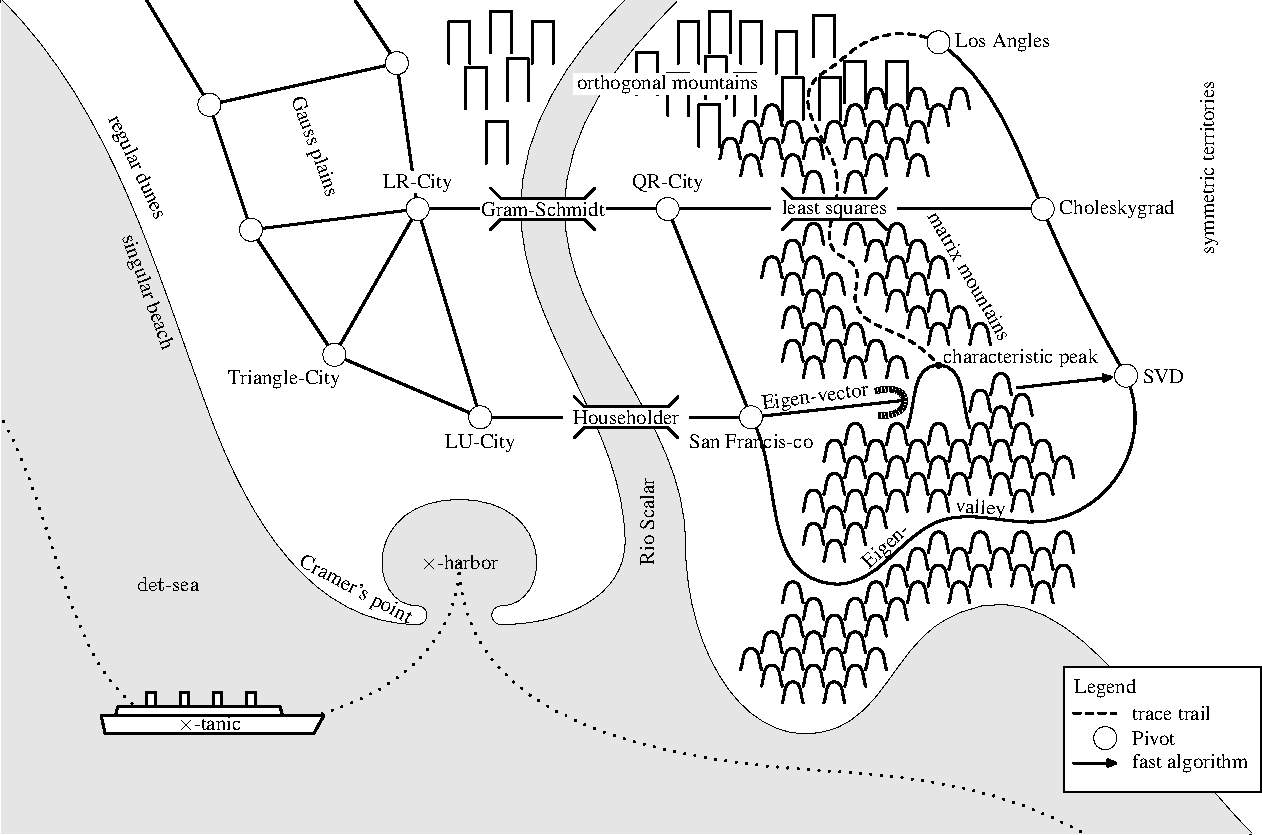
\includegraphics[width=0.95\hsize]{images/linalgmap-1}
\end{center}
\end{landscape}

%
% part1.tex -- Teil 1 über Struktur in der Mathematik
%
% (c) 2017 Prof Dr Andreas Müller, Hochschule Rapperswil
%
\part{Struktur}

\chapter*{Mathematische Strukturen}


Die Betonung der zugrunde liegenden mathematischen Strukturen ist
ein besonderes Kennzeichen der Mathematik des zwanzigsten und 
einzundzwanzigsten Jahrhunderts und verdient daher im ersten Teil
etwas genauer studiert zu werden.


%
% vektorraum.tex
%
% (c) 2017 Prof Dr Andreas Müller, Hochschule Rapperswil
%
\chapter{Vektorraum}
Wenn angehende Ingenieure zum ersten Mal mit linearer Algebra in
Kontakt kommen, arbeiten sie meistens mit Spaltenvektoren von
reellen Zahlen.
Diese Vektoren können mit reellen Zahlen multipliziert werden,
Vektoren können addiert und subtrahiert werden.
Später kommen Matrizen hinzu, welche oft als eine rein formale
Erweiterung der Vektoren betrachtet werden können, als ``dicke''
Vektoren, für die es eine zusätzliche Verknüpfung mit Vektoren
gibt.
Entsprechend liegt das Schwergewicht oft auf Anwendungen in der
Vektorgeometrie.

Dabei gerät oft in Vergessenheit, dass auch ein viel grösseres
Anwendungsgebiet zum Beispiel in der Analysis oder der Kryptographie
haben.
Auch Funktionen können addiert, subtrahiert und mit reellen Zahlen
multipliziert werden.
Auch für Funktionen kann man ein Skalarprodukt definieren, und
damit die geometrisch Idee der orthonormierten Basis und der
einfachen Zerlegung bezüglich einer Basis für Funktionen nutzen,
dies ist die geometrische Betrachtungsweise der Fourier-Theorie.

Damit man die Erkenntnisse der linearen Algebra in dieser Form
nutzen kann, muss man sich erst von der Fixierung auf Spaltenvektoren
lösen.
Man muss also die grundlegende Theorie zuerst so abstrakt formulieren,
dass sie tatsächlich auf die genannten Situationen angewendet werden 
kann.


%
% skalare.tex
%
% (c) 2017 Prof Dr Andreas Müller, Hochschule Rapperswil
%
\section{Skalare -- Körper}
In der elementaren lineare Algebra können Vektoren mit reellen
Zahlen multipliziert werden, Zahlen können mit Zahlen multiplizert
werden, Vektoren mit Vektoren, aber es gibt keine Multiplikation
von Vektoren.
Ausserdem kann man natürlich durch beliebige reelle Zahlen teilen,
eine wesentliche Voraussetzung für die Lösung von linearen Gleichungssysteme.
Die lineare Algebra unterscheidet also Objekte, die nicht miteinander
multipliziert werden können und solche, für die alle arithmetischen
Operationen möglich sind.

Die reellen Zahlen haben aber noch viel mehr Struktur, welche in
der linearen Algebra nicht benötigt werden.
Zum Beispiel können positive und negative reelle Zahlen unterschieden
werden, eine Eigenschaft, die für die Lösung linearer Gleichungssyteme
irrelevant zu sein scheint.
Jede Cauchy-Folge reeller Zahlen hat einen Grenzwert, doch das Konzept
des Grenzwertes spielt in der elementaren linearen Algebra ebenfalls
keine Rolle.

Ziel dieses Kapitel ist daher, die tatsächlich nötigen, minimalen
Anforderungen an die Skalare in der linearen Algebra zu formulieren.
Dabei wird die Struktur des Zahlkörpers in den Vordergrund gerückt
und weitere Beispiele von Zahlkörpern werden besprochen.
Der Fall der endlichen Körper wird im Kapitel~\ref{chapter:endlichekoerper}
im Detail untersucht.

\subsection{Skalare}
Welche Operation nötig sind, um lineare Gleichungssysteme zu lösen
verraten schon das einfachsten lineare Gleichungsysteme.
Aus dem $1\times 1$-Gleichungssystem 
\[
ax=b\qquad\Rightarrow\qquad x=\frac{b}{a}
\]
folgt, dass man durch beliebige von $0$ verschiedene Elemente dividieren
können muss.
Das Gleichungssystem
\[
\left.
\begin{linsys}{3}
ax&+&by&=&c\\
  & &dy&=&e
\end{linsys},
\right\}
\qquad\Rightarrow\qquad
y=\frac{e}{d},\quad
x=\frac1{a}\biggl(c-b\frac{e}{d}\biggr)
\]
kann nur gelöst werden, wenn auch die Subtraktion zur Verfügung steht.
Eine im Sinne des Ziels der Lösung linearer Gleichungen sinnvolle 
Theorie kann also nur aufgebaut werden, wenn alle arithmetischen
Grundoperationen zur Verfügung stehen.

Mehr als die arithmetischen Grundoperationen ist erst dann nötig, 
wenn man Eigenwerte bestimmen will. 
Dann müssen zum Beispiel Nullstellen des charakteristischen Polynoms
bestimmt werden.
Doch einfache Bespiele zeigen, dass dies nicht einmal in den reellen
Zahlen immer möglich ist.
Das Ziel muss daher sein, Zahlenmengen zu charakterisieren, die die
Rolle der Skalare in der linearen Algebra übernehmen können.
Eine solche Menge muss die Lösung beliebiger lineare Gleichungssysteme
ermöglichen, wir verlangen aber nicht, dass auch beliebige Eigenwertprobleme
gelöst werden können.

\subsection{Körper}
Die folgende Definition beschreibt eine Zahlenmenge, in der alle
Grundoperationen zur Verfügung stehen, eine solche Menge heisst
ein {\em Körper}.
\index{Körper}%

\begin{definition}
Sei $K$ eine Menge mit zwei Operationen, der Addition, geschrieben $+$,
und der Multiplikation, geschrieben $\cdot$, die die folgenden
Eigenschaften hat:
\begin{compactenum}
\item Die Addition ist assoziativ und kommutativ.
\item Es gibt ein neutrales Element $0\in K$ für die Addition,
d.~h.~$a+0=a$ für alle $a\in K$.a
\item Jede Gleichung $x+a=b$ mit $a,b\in K$ kann eindeutig nach $x$ aufgelöst
werden.
\item Die Multiplikation ist assoziativ und kommutativ.
\item Es gibt ein neutrales Element $1$ für die Multiplikation,
d.~h.~$1\cdot a=a$ für alle $a\in K$.
\item Jede Gleichung $ax=b$ mit $a,b\in K$ und $a\ne 0$ kann eindeutig 
nach $x$ aufgelöst werden, die Lösung wird $x=b/a=ba^{-1}$ geschrieben.
\item Für beliebige $a,b,c\in K$ gilt
$a(b+c)=ab+ac$.
\end{compactenum}
$K$ heisst ein {\em Körper}.
\end{definition}

Die Forderung nach Assoziativität stellt sicher, dass Summen oder
Produkte mit mehr als zwei Summanden bzw.~Faktoren in beliebiger
Reihenfolge berechnet werden können.

Die Forderung nach Kommutativität sieht im Moment vor allem nach
Bequemlichkeit aus.
Eine genauere Analyse des Gauss-Algorithmus zeigt jedoch, dass er 
nur für kommutative Skalare funktioniert.

Die Bedingung 3 definiert die Subtraktion während Bedingung 6
besagt, dass man auf eindeutige Art durch von $0$ verschiedene
Zahlen teilen kann.

Die Bedingung~7, das Distributivgesetz, stellt sicher,
dass die algebraischen Operationen
sich so verhalten, wie man es sich aus der Schule kennt.
Zum Beispiel kann die Gleichug $ax+b=c$ auf zwei Arten gelöst werden
\begin{align*}
\xymatrix{
\txt{}	&{ay+b=c}\ar[dr]\ar[dl]
\\
ay=c-b \ar[d]	&\txt{}	&y+ba^{-1}=ca^{-1}\ar[d]
\\
y=(c-b)a^{-1}&\txt{}&	y=ca^{-1}-ba^{-1}
}
\end{align*}
Auf dem linken Ast wir erst die Konstante $b$ auf die rechte Seite
gebracht, auf dem rechten wird erst durch $a$ dividiert.
Natürlich sollten beide Lösungen übereinstimmen, dies ist nur möglich,
wenn das Distributivgesetz gilt.

\subsection{Beispiele}
Die reellen Zahlen bilden ganz offensichtlich einen Körper.
Andererseits bilden die ganzen Zahlen ganz bestimmt keinen Körper,
denn die Gleichung $2x=1$ hat keine ganzzahlige Lösung, im Widerspruch
zu Eigenschaft~6 eines Körpers.
Auch die natürlichen Zahlen bilden keinen Körper, denn die Gleichung
$x+1=0$ hat keine Lösung in $\mathbb N$, im Widerspruch zur Eigenschaft~3
eines Körpers.
In diesem Kapitel sollen daher ein paar Beispiele von Köpern
zusammengestellt werden.

\subsubsection{Rationale Zahlen}
Die rationalen Zahlen $\mathbb Q$ erweitern die ganzen Zahlen $\mathbb Z$
so, dass beliebige Divisionen durchführen kann.
Die rationalen Zahlen bilden den kleinsten Körper, der die ganzen
Zahlen enthält.
Die ganze lineare Algebra liesse sich also auch ausschliesslich in
den rationalen Zahlen entwickeln.

\subsubsection{Quotientenkörper eines Ringes}
Die rationalen Zahlen enstanden dadurch, dass aus ganzen Zahlen $\mathbb Z$
Brüche konstruiert wurden.
Wenn wir die Elemente der Menge
\[
\{ (z,n)\,| z,n\in\mathbb Z\wedge n\ne 0\}
\]
als Brüche betrachten wollen, dann müssen wir zwei Brüche
$(z_1,n_1)$ und $(z_2,n_2)$ als gleich betrachten, wenn sie
übereinstimmen, sobald man sie gleichnamig gemacht hat.
Multipliziert man $(z_1,n_1)$ mit $n_2$ und $(z_2,n_2)$ mit $n_1$, dann
beschreiben die erweiterten Brüche
$(z_1n_2,n_1n_2)$ und $(z_2n_1,n_1n_2)$ die gleiche Zahl, wenn
$z_1n_2=z_2n_1$.
Eine rationale Zahl $q=z/n$ kann also betrachtet werden als die
Teilmenge
\[
q
=
M(q)
=
\{(z',n')\,|\, z',n'\in\mathbb Z\wedge n'\ne 0 \wedge zn'=z'n\}
\subset
\{(z',n')\,|\, z',n'\in\mathbb Z\wedge n'\ne 0\}.
\]
Die Menge der $M(q)$ kann betrachtet werden als die Menge der rationalen
Zahlen.

Diese Konstruktion kann verallgemeinert werden, wie wir an einem
Beispiel illustrieren wollen.
Sei $R=\mathbb R[X]$ die Menge der Polynome in der Variablen $X$
mit reellen Koeffizienten.
Die Axiome eines Körpers sind für $R$ nicht alle erfüllt.
Bedingung~6 ist nicht erfüllt, da man im Allgemeinen nicht durch Polynome
dividieren kann.

Motiviert durch die Konstruktion der Brüche kann man jedoch die Menge
der Brüche von Polynomen konstruieren.
Dazu betrachtet man zunächst die Menge
\[
\{ (p,q)\,|\, p,q\in \mathbb R[X]\wedge q\ne 0\}
\]
von Paaren von Polynomen.
Dann bildet man für ein vorgegebenens Paar von Polynomen $r=(p,q)$ die
Teilmenge
\[
M(r)
=
\{ (p',q')\,|\, p',q'\in \mathbb R[X]\wedge q'\ne 0\wedge pq'=p'q\}.
\]
Die Menge $M(r)$ besteht aus allen Polynombrüchen, die nach 
Gleichnamigmachen mit $q$ übereinstimmen.
Wir nennen die Menge 
\[
\mathbb R(X)
=
\{ M(r)\, |\, r=(p,q)\wedge p,q\in\mathbb R[X]\wedge q\ne 0\}
\]
die Menge der rationalen Funktionen in der Variablen $X$, sie ist
ein Körper.
Wir verwenden im Folgenden wieder die üblichere Schreibweise $p(X)/q(X)$
für $r\in\mathbb R(X)$.

Die Konstruktion der Brüche funktioniert, solange die Operation des
Gleichnamigmachens wohldefiniert ist.
Dazu ist zunächst notwendig, dass bleibige Multiplikationen ausführbar
sind.
Eine Menge $R$, die alle Axiome eines Körpers ausser 5 und 6 erfüllt,
heisst ein kommutativer Ring.

Dann ist notwendig, dass die Multiplikation der Nenner nie auf $0$ führt.
Man nennt $R$ einen {\em Integritätsbereich},
wenn $n_1n_2\ne 0$ für beliebige $n_1,n_2\ne 0$.
\index{Integritätsbereich}%
Die Konstruktion der Brüche ist also möglich für beliebige
Integritätsbereiche.

\subsubsection{Komplexe Zahlen}
Die Menge $\mathbb C$ der komplexen Zahlen entstehen aus der Menge $\mathbb R$
der reellen Zahlen dadurch, dass man ein neues Element $i$ mit der Eigenschaft
$i^2=-1$ hinzufügt, dabei aber alle anderen Rechenregeln beibehält.
Da das Quadrat von $i$ wieder eine reelle Zahl ist, kann man jede beliebige
komplexe Zahl in der Form $a+bi$ schreiben.
Es stellt sich heraus, dass man in der Menge der komlexen Zahlen beliebig
divideren kann:
\[
\frac{a+bi}{c+di}
=
\frac{a+bi}{c+di}
\cdot
\frac{c-di}{c-di}
=
\frac{ac-bd + i(ad+bc)}{c^2 + d^2},
\]
natürlich nur, wenn $c^2+d^2\ne 0$ oder $c+di\ne 0$.
Die Menge $\mathbb C$ ist also ein Körper.

Die besondere Bedeutung der komplexen Zahlen für die lineare Algebra ist, 
dass darin nicht nur Gleichungssyteme gelöst werden können.
In $\mathbb C$ kann auch jede Polynomgleichung gelöst werden, so dass
sich das Eigenwertproblem immer lösen lässt.

\subsubsection{Endliche Körper}
In der Menge $\mathbb F_p=\mathbb F_5$ der Reste bezüglich der Primzahl
$p=5$ sind die Addition und die Multiplikation wohldefiniert.
Die Additions- und Multiplikationstabellen sind
\[
\begin{tabular}{|c|ccccc|}
\hline
$+$&0&1&2&3&4\\
\hline
0&0&1&2&3&4\\
1&1&2&3&4&0\\
2&2&3&4&0&1\\
3&3&4&0&1&2\\
4&4&0&1&2&3\\
\hline
\end{tabular}
\qquad
\begin{tabular}{|c|ccccc|}
\hline
$\cdot$&0&1&2&3&4\\
\hline
0&0&0&0&0&0\\
1&0&1&2&3&4\\
2&0&2&4&1&3\\
3&0&3&1&4&2\\
4&0&4&3&2&1\\
\hline
\end{tabular}
\]
Da in jeder Zeile jede Zahl genau einmal vorkommt (ausser in den ersten
Zeilen und Spalte in der Multiplikationstabelle) kann man schliessen, dass
die Menge $\mathbb F_5$ die Bedingungen 3 und 6 eines Körpers erfüllt.
Somit ist $\mathbb F_5$ ein Körper.
Es gilt sogar allgemein für jede beliebige Primzahl, dass die Menge
$\mathbb F_p$ ein Körper ist.
Im Gegensatz zu den bereits untersuchten Körpern ist $\mathbb F_p$ endlich.
Die lineare Algebra in endlichen Körpern wird in
Kapitel~\ref{chapter:endlichekoerper} genauer untersucht.

Allerdings lassen sich nicht alle Polynomgleichungen mit Koeffizienten
in $\mathbb F_5$ lösen.
Die Gleichung
\[
x^2-2=0
\]
hat keine Lösung in $\mathbb F_5$, wie man durch Inspektion der
Multiplikationstabelle einsehen kann.


\subsection{Körpererweiterungen}
Die Körper der rationalen Zahlen und der reellen Zahlen sind insofern
nicht optimal für die lineare Algebra, dass sich das Eigenwertproblem
nicht immer lösen lässt.
Dabei wäre es nur nötig, dass der Körper die Nullstellen des
charakteristischen Polynoms enthält. 
Die Matrix
\[
J=\begin{pmatrix}0&-1\\1&0\end{pmatrix}
\]
hat das charakteristische Polynom
\[
\varphi_{J}(\lambda)
=
\left|\begin{matrix}-\lambda&-1\\1&-\lambda\end{matrix}\right|
=
\lambda^2+1 = 0
\qquad\Rightarrow\qquad
\lambda=\pm i.
\]
Die Eigenwerte von $J$ sind also nicht im Körper enthalten,
und damit können auch die Eigenvektoren nicht reell sein.

Betrachtet man $J$ dagegen als komplexe Matrix, lassen sich sofort
Eigenvektoren für die Eigenwerte $\pm i$ angeben.
Dazu verwendet man den Gauss-Algorithmus auf die Matrix $J\pm iI$ an:
\[
\begin{aligned}
\begin{tabular}{|>{$}c<{$}>{$}c<{$}|>{$}c<{$}|}
\hline
         - i&-1&0\\
\phantom{-}1&-i&0\\
\hline
\end{tabular}
&\rightarrow
\begin{tabular}{|>{$}c<{$}>{$}c<{$}|>{$}c<{$}|}
\hline
 1&         - i&0\\
 0&\phantom{-}0&0\\
\hline
\end{tabular}
&&\Rightarrow
&
v_+&=\begin{pmatrix}i\\1\end{pmatrix},
&
Jv_+&=\begin{pmatrix}-1\\i\end{pmatrix}
=
i\begin{pmatrix}i\\1\end{pmatrix}
=
iv_+,
\\
\begin{tabular}{|>{$}c<{$}>{$}c<{$}|>{$}c<{$}|}
\hline
\phantom{-}i&         - 1&0\\
\phantom{-}1&\phantom{-}i&0\\
\hline
\end{tabular}
&\rightarrow
\begin{tabular}{|>{$}c<{$}>{$}c<{$}|>{$}c<{$}|}
\hline
 1&\phantom{-}i&0\\
 0&\phantom{-}0&0\\
\hline
\end{tabular}
&&\Rightarrow
&
v_-&=\begin{pmatrix}-i\\1\end{pmatrix},
&
Jv_-&=\begin{pmatrix}1\\i\end{pmatrix}
=
-i\begin{pmatrix}-i\\1\end{pmatrix}
=
-iv_-.
\end{aligned}
\]
Das Eigenwertproblem ist also vollständig lösbar geworden, indem
man dem ursprünglichen Körper genau die fehlenden Elemente, in diesem
Fall $i$ und $-i$ hinzugefügt hat, und wieder dafür gesorgt hat, dass
man einen Körper hat.
So ist der Körper $\mathbb C$ entstanden.

Man kann die Matrix $J$ aber auch als rationale Matrix betrachten.
Nach den eben gezeigten Lösung des Eigenwertproblems müsste es also
reichen, den rationalen Zahlen $\mathbb Q$ nur die imaginäre Einheit $i$
hinzuzufügen.
So erhält man eine Teilmenge
\[
\mathbb Q(i) = \{a+bi\,|\, a,b\in\mathbb Q\} \subset \mathbb C
\]
der komplexen Zahlen mit rationalen Komponenten.
Damit haben wir einen neuen Körper zwischen $\mathbb Q$ und $\mathbb C$
gefunden, der gross genug ist, das Eigenwertproblem für $J$ zu lösen.

\subsubsection{Körpererweiterung von $\mathbb Q$}
Wir versuchen dasselbe Vorgehen für das Eigenwertproblem für die Matrix
\[
A
=
\begin{pmatrix}
3&1\\
1&1
\end{pmatrix}.
\]
Die rationale Matrix $A$ hat das charakteristische Polynom
\[
\chi_{A}(\lambda)
=
\left|\begin{matrix}3-\lambda&1\\1&1-\lambda\end{matrix}\right|
=
(3-\lambda)(1-\lambda)-1
=
\lambda^2-4\lambda+2
\]
mit den Nullstellen
\[
\lambda_{\pm} = 2\pm\sqrt{4-2}=2\pm\sqrt{2} \not\in \mathbb Q.
\]
Zwischen den Zahlen $\lambda_+$ und $\lambda_-$ besehen die Beziehungen
\begin{align*}
\lambda_+ + \lambda_-=4
\quad&\Rightarrow\quad \lambda_-=4-\lambda_+
\\
\lambda_+\lambda_- = 2
\quad&\Rightarrow\quad \lambda_-=\frac{2}{\lambda_+}.
\end{align*}
Fügen wir die Zahl $\lambda_+$ den rationalen Zahlen hinzu sowie alle
Zahlen, die sich mit Hilfe der Körperoperationen daraus bilden lassen,
dann erhalten wir einen Körper, den wir
\[
\mathbb Q(2+\sqrt{2})
=
\{ a+b(2+\sqrt{2})\,|\, a,b\in\mathbb Q\}
=
\{ a + b\sqrt{2}\,|\,a,b\in\mathbb Q\}
=
\mathbb Q(\!\sqrt{2})
\]
bezeichnen.
In diesem Körper können wir jetzt das Eigenwertproblem für die Matrix $A$
lösen:
\[
\begin{aligned}
\begin{tabular}{|>{$}c<{$}>{$}c<{$}|}
\hline
3-\lambda_+&1          \\
1          &1-\lambda_+\\
\hline
\end{tabular}
&=
\begin{tabular}{|>{$}c<{$}>{$}c<{$}|}
\hline
1-\sqrt{2}& 1         \\
1         &-1-\sqrt{2}\\
\hline
\end{tabular}
\rightarrow
\begin{tabular}{|>{$}c<{$}>{$}c<{$}|}
\hline
1&-1-\sqrt{2}\\
0&0          \\
\hline
\end{tabular}
&&\Rightarrow&v_+&=\begin{pmatrix}1+\sqrt{2}\\1\end{pmatrix}
\\
\begin{tabular}{|>{$}c<{$}>{$}c<{$}|}
\hline
3-\lambda_-&1          \\
1          &1-\lambda_-\\
\hline
\end{tabular}
&=
\begin{tabular}{|>{$}c<{$}>{$}c<{$}|}
\hline
1+\sqrt{2}& 1         \\
1         &-1+\sqrt{2}\\
\hline
\end{tabular}
\rightarrow
\begin{tabular}{|>{$}c<{$}>{$}c<{$}|}
\hline
1&-1+\sqrt{2}\\
0&0          \\
\hline
\end{tabular}
&&\Rightarrow&v_-&=\begin{pmatrix}-1+\sqrt{2}\\1\end{pmatrix}
\end{aligned}
\]
Die Vektoren $v_+$ und $v_-$ haben Komponenten in $\mathbb Q(\!\sqrt{2})$.

Damit haben wir ein allgemeines Prinzip gefunden
für die Lösung von Eigenwertproblemen in Körpern $K$,
welche die Nullstellen des charakteristischen Polynoms noch
nicht enthalten. 
Wir erweitern den Körper um die Nullstellen $\lambda_1,\dots,\lambda_n$
und erhalten einen neuen Körper
\[
K(\lambda_1,\dots,\lambda_n),
\]
der alle $\lambda_i$ enthält und alle Zahlen, die sich daraus durch
arithmetische Operationen bilden lassen.
In diesem Körper lässt sich das Eigenwertproblem lösen.
Man nennt $K(\lambda_1,\dots,\lambda_n)$ eine Körpererweiterung von $K$.
\index{Körpererweiterung}%

Im Lichte dieser Prozedur erklärt sich die besondere Bedeutung
von $\mathbb C$ wie folgt. 
Man muss dem Körper $\mathbb R$ nur die Zahl $i$ hinzufügen um
den Körper $\mathbb R(i)=\mathbb C$ zu erhalten, in dem sich alle Nullstellen
von beliebigen reellen Polynomen befinden.
Die komplexen Zahlen bilden also einen universellen Körper, in dem
sich jede Polynomgleichung lösen lässt.
Man nennt $\mathbb C$ {\em algebraisch abgeschlossen}.
\index{algebraisch abgeschlossen}%
In einem algebraisch abgeschlossenen Körper lässt sich jedes Eigenwertproblem
lösen.

\subsubsection{Körpererweiterung eines endlichen Körpers}
Auch bei endlichen Körpern funktioniert die Körpererweiterungsidee.
Wir versuchen das Eigenwertproblem für die Matrix $A$ in $\mathbb F_5$ 
zu lösen.
Das charakteristische Polynom ist
\[
\chi_{A}(\lambda) = \lambda^2 + \lambda + 2,
\]
es hat keine Nullstellen in $\mathbb F_5$.
Sei $\alpha$ eine Zahl, welche Nullstelle des charakteristishen Polynoms ist,
der erste Eigenwert ist daher $\lambda_1=\alpha$.
Aus dem charakteristischen Polynom folgt, dass $\alpha^2=-\alpha-2$.
Dann ist die zweite Nullstelle $\lambda_2=-(\alpha+1)=4(\alpha+1)$,
wie man durch Ausmultiplizieren 
\begin{align*}
(\lambda-\alpha)(\lambda + (\alpha+1))
&=
\lambda^2 -\alpha\lambda +(\alpha+1)\lambda -\alpha(\alpha+1)
=
\lambda^2 + \lambda-\alpha^2-\alpha
\\
&=
\lambda^2 + \lambda + \alpha + 2 - \alpha
=
\lambda^2 + \lambda + 2
=
\chi_{A}(\lambda)
\end{align*}
nachprüfen kann.
Dann kann man Eigenvektoren wieder mit dem Gaussalgorithmus ermitteln
\[
\begin{aligned}
\begin{tabular}{|>{$}c<{$}>{$}c<{$}|}
\hline
3-\alpha &1       \\
1        &1-\alpha\\
\hline
\end{tabular}
&\rightarrow
\begin{tabular}{|>{$}c<{$}>{$}c<{$}|}
\hline
1        &1-\alpha\\
0        &0       \\
\hline
\end{tabular}
&&\Rightarrow
&v_1&=\begin{pmatrix}-1+\alpha\\ 1 \end{pmatrix},
\\
\begin{tabular}{|>{$}c<{$}>{$}c<{$}|}
\hline
3+\alpha+1 &1       \\
1        &1+\alpha+1\\
\hline
\end{tabular}
=
\begin{tabular}{|>{$}c<{$}>{$}c<{$}|}
\hline
\alpha-1 &1       \\
1        &2+\alpha\\
\hline
\end{tabular}
&\rightarrow
\begin{tabular}{|>{$}c<{$}>{$}c<{$}|}
\hline
1        &2+\alpha\\
0        &0       \\
\hline
\end{tabular}
&&\Rightarrow
&v_2&=\begin{pmatrix}3+4\alpha\\ 1 \end{pmatrix}.
\end{aligned}
\]
Ebenfalls durch Ausmultiplizieren kann man nachprüfen, dass dies tatsächlich
Eigenvektoren sind.
Damit haben wir gezeigt, dass im Erweiterungskörper $\mathbb F_5(\alpha)$
das Eigenwertproblem für die Matrix $A$ gelöst werden kann.
$\mathbb F_5(\alpha)$ spielt also die gleiche Rolle für $\mathbb F_5$, wie
sie $\mathbb Q(\!\sqrt{2})$ für $\mathbb Q$ spielt.


%
% vektoren.tex -- Vektoren
%
% (c) 2017 Prof Dr Andreas Müller, Hochschule Rapperswil
%
\section{Vektoren}
\rhead{Vektoren}
Die zweite Zutat zu der Struktur, die wir in diesem Kapitel
konstruieren wollen, sind die Vektoren.
Wir gehen wieder wie bei den Skalaren vor un formulieren nur
die unbedingt nötigen Anforderungen in Form von Axiomen.
Dann zeigen wir neue Beispiele von Vektorräumen, was illustrieren soll,
dass die abstrakte Theorie erlaubt, auf vereinheitlichte Weise über
verschiedene Arten von Vektoren Erkenntnisse zu gewinnen.

\subsection{Axiome eines Vektorraumes}
Die Vektoren bilden eine Menge, in der man Addition und Subraktion 
ausführen kann.
Ausserdem kann man Vektoren mit Skalaren aus einem Körper $K$ multiplizieren.

\begin{definition}
Eine Vektorraum über dem Körper $K$ oder $K$-Vektorraum
ist eine Menge $V$, genannt die Vektoren,
mit einer kommutativen und assoziativen Operation $+$ und einer Multiplikation
von Skalaren mit Vektoren, mit folgenden Eigenschaften
\begin{compactenum}
\item Die Operationen sind assoziativ: $(\lambda\mu)v=\lambda(\mu v)$ für
$\lambda,\mu\in K$ und $v\in V$.
\item Es gibt neutrales Element der Addition $0\in V$, es gilt also
$0+v=v$ für $v\in V$.
\item Jede Gleichung $x+u=v$ mit $u,v\in V$ hat eine eindeutige Lösung
$x=v-u\in V$.
\item Für die Multiplikation gilt $1\cdot v=v$ für alle $v\in V$.
\item Die Operationen sind miteinander verträglich im Sinne der 
Distributivgesetze:
\begin{align*}
(\lambda + \mu)v&=\lambda v + \mu v
\\
\lambda(u+v)&=\lambda u + \lambda v
\end{align*}
für $u,v\in V$ und $\lambda,\mu\in K$.
\end{compactenum}
\end{definition}

\subsection{Beispiele}
Das offensichtliche Beispiel der Zeilen- oder Spalten-Vektoren wollen wir
hier nicht erneut besprechen.

\subsubsection{Polynome}
Ist $K$ ein Körper, dann sei
\[
K[X]
=
\{
a_0+a_1X+\dots a_nX^n\,|\, a_0,\dots,a_n\in K
\}
\]
die Menge aller Polynome mit Koeffizienten in $K$.
$K[X]$ ist ein Vektorraum, denn man kann offenbar Polynome addieren und
mit Skalaren aus $K$ multiplizieren.
Die Addition ist kommutativ und das Polynom $0\in K[X]$ ist ihr neutrales
Element.
Die Vektorraumaxiome sind nichts anders als die üblichen Rechenregeln
für Polynome.

Man bemerkt, dass $K[X]$ sogar eine kommutative Multiplikation hat
mit dem neutralen Element $1$.
$K[X]$ ist also ein Ring und sogar ein Integritätsbereich, es lässt sich
also der Quotientenkörper $K(X)$ der rationalen Funktionen mit Koeffizienten
in $K$ konstruieren.

\subsubsection{Stetige Funktionen}
Die Menge
\[
C([a,b])
=
\{ f\colon [a,b]\to \mathbb R\;|\; \text{$f$ ist stetig}\},
\]
ist ein $\mathbb R$-Vektorraum.
Funktionen können punktweise addiert und mit reellen Skalaren multipliziert
werden, wenn man definiert
\[
\begin{aligned}
(f+g)(x)&=f(x)+g(x)
&&\text{und}
&
(\lambda f)(x)&=\lambda f(x)
\end{aligned}
\]
für $f,g\in C([a,b])$ und $\lambda\in\mathbb R$.

Auch in diesem Fall ist $C([a,b])$ ein Ring mit der konstanten Funktion $1$
als neutrales Element der Multiplikation.
Allerdings ist dieser Ring nicht ein Integritätsbereich, da das Produkt der
beiden stetigen Funktionen
\[
f(x)
=
\begin{cases}
0&\qquad x<\displaystyle\frac{a+b}2\\
\displaystyle x-\frac{a+b}2&\qquad x\ge \displaystyle\frac{a+b}2
\end{cases}
\qquad\text{und}\qquad
g(x)
=
\begin{cases}
\displaystyle\frac{a+b}2-x&\qquad x<\displaystyle\frac{a+b}2\\
0&\qquad x\ge \displaystyle\frac{a+b}2
\end{cases}
\]
verschwindget: $(fg)(x)=f(x)g(x)=0$.
Damit ist die Konstruktion des Quotientenkörpers nicht möglich.
Dies illustriert, dass die algebraische Struktur der Polynome viel
rigider ist als die der stetigen Funktionen.

Die Menge $C([a,b])$ trägt aber noch zusätzliche Struktur, welche
wir erst später untersuchen können.
Es ist möglich, auf $C([a,b])$ eine Norm zu definieren, und damit
Cauchy-Folgen und Grenzwerte zu definieren.
Dies ist möglich auf eine Art, dass Grenzwerte von stetigen Funtionen
existieren und wieder stetige Funktionen sind.
So etwas ist für Polynome nicht möglich, da man jede beliebige stetige
Funktion beliebig genau mit Polynomen approximieren kann.
Wir können den Polynomring daher als einen Teilvektorraunm
$\mathbb R[X]\subset C([a,b])$ betrachten.

\subsection{Lineare Abhängigkeit}
Sind $v_i,b\in V$ Vektoren, dann ist
\begin{equation}
x_1 v_1 + \dots + x_n v_n = b
\label{vektorraum:lingl}
\end{equation}
ein lineares Gleichungssystem für die Zahlen $x_1,\dots,x_n\in K$.
Die linke Seite von \eqref{vektorraum:lingl} heisst eine
{\em Linearkombination} der Vektoren $v_1,\dots,v_n$.
In diesem Moment interessiert uns nicht die Frage, wie man dieses
Gleichungsssystem löst, sondern die Frage, ob das Gleichungssystem
übrerhaupt lösbar ist.

Je nach rechter Seite $b$ könnte es gar keine Lösung der Gleichung
\eqref{vektorraum:lingl} geben.
Dieses Phänomen ist bekannt aus der elementaren Theorie, nur wenn
\[
b\in \{ x_1v_1+\dots+ x_nv_n\,|x_i\in K\}
=
\operatorname{span}(v_1,\dots,v_n)
=
\langle v_1,\dots,v_n\rangle,
\]
gilt, wird das Gleichungssystem eine Lösung haben.
Die Menge auf der rechten Seite ist ein Unterraum von $V$ und
heisst das {\em Erzeugnis} der Vektoren $v_1,\dots,v_n$ oder
\index{Erzeugnis}%
der von $v_1,\dots,v_n$ {\em aufgespannte} Vektorraum.
\index{aufgespannter Vektorraum}%
Die Bedingung ist aber auf jeden Fall erfüllt für $b=0$, 
eine Lösung kann man dann auch unmittelbar angeben:
$(x_1,\dots,x_n)=(0,\dots,0)$.

Es bleibt die Frage, ob die Lösung eindeutig bestimmt ist.
Nehmen wir an, dass es zwei Lösungen $(x_1,\dots,x_n)$ und
$(x_1',\dots,x_n')$ des Gleichungssystems \eqref{vektorraum:lingl}
gibt.
Für beide Lösung gilt die Gleichung:
\begin{align*}
x_1v_1+\dots+x_nv_n&=b\\
x_1'v_1+\dots+x_n'v_n&=b
\end{align*}
Die Differenz ist dann
\begin{equation}
(x_1-x_1')v_1+\dots + (x_n-x_h') v_n = 0
\label{vektorraum:diffgl}
\end{equation}
Die Gleichung
\eqref{vektorraum:lingl} ist also genau dann eindeutig lösbar
wenn die Gleichung \eqref{vektorraum:diffgl} nur mit den Werten
\[
\begin{aligned}
x_1-x_1'&=0,&&\dots,&
x_n-x_n'&=0
\end{aligned}
\]
befriedigt werden kann.
Wir fassen dies zusammen im Begriff der linearen Unabhängigkeit.

\begin{definition}
Die Vektoren $v_1,\dots,v_n$ heissen {\em linear unabhängig}, wenn die
Gleichung
\[
\lambda_1v_1 + \dots + \lambda_nv_n=0
\]
nur die Lösung $\lambda_1=\dots=\lambda_n=0$ hat.
\end{definition}
\index{linear abhängig}

Ein lineares Gleichungssystem der Form \eqref{vektorraum:lingl}
kann als nur dann eindeutig lösbar sein, wenn die Vektoren
$v_1,\dots,v_n$ linear unabhängig sind.
Eine Lösung wird nur existieren, wenn die Vektoren
$v_1,\dots,v_n,b$ linear abhängig sind.



%
% lineareabbildung.tex
%
% (c) 2017 Prof Dr Andreas Müller, Hochschule Rapperswil
%
\section{Linear Abbildungen}
In diesem Abschnitt betrachten wir zwei Vektorräume $U$ und $V$ und
eine Abbildungen $f\colon U\to V$, welche mit der Vektorraumstruktur
verträglich sein soll. 
Dazu muss für zwei Vektoren $u_1,u_2\in U$ und für $\lambda\in K$ gelten
\begin{equation}
f(u_1+u_2)=f(u_1)+f(u_2)
\qquad\text{und}\qquad
f(\lambda u_1)=\lambda f(u_1).
\label{vektorraum:linear}
\end{equation}
Wir können diese Eigenschaft in einer einzigen Formel zusammenfassen:

\begin{definition}
Eine Abbildung $f\colon U\to V$ heisst linear, wenn gilt
\[
f(\lambda_1 u_1+\lambda_2 u_2)=\lambda_1 f(u_1) + \lambda_2 f(u_2)
\]
für alle $u_1,u_2\in U$ und $\lambda_1,\lambda_2\in K$.
\end{definition}

Die Formeln~\eqref{vektorraum:linear} sind Spezialfälle der Definition.
Die Menge der linearen Abbildungen ist selbst wieder ein Vektorraum.

\begin{definition}
Seien $U$ und $V$ Vektorräume über $K$, dann ist
\[
L(U,V)
=
\operatorname{Hom}(U,V)
=
\{f\colon U\to V\;|\; \text{$f$ ist linear}\}
\]
der Vektorraum der linearen Abbildungen von $U$ nach $V$.
\end{definition}

Wir müssen nachprüfen, dass lineare Abbildungen tatsächlich einen
Vektorraum bilden. 
Dazu muss zunächst überprüft werden, ob die Summe linearer Abbildungen
wieder linear ist.
Tatsächlich ist
\begin{align*}
(f_1+f_2)(\lambda_1u_1+\lambda_2 u_2)
&=
f_1(\lambda_1u_1+\lambda_2 u_2)
+
f_2(\lambda_1u_1+\lambda_2 u_2)
\\
&=
\lambda_1f_1(u_1)+\lambda_2f_1(u_2)
+
\lambda_1f_2(u_1)+\lambda_2 f_2(u_2)
\\
&=
\lambda_1(f_1 + f_2)(u_1)+\lambda_2(f_1+f_2)(u_2),
\\
(\lambda f)(\lambda_1 u_1 + \lambda_2 u_2)
&=
\lambda (f(\lambda_1 u_1 + \lambda_2 u_2))
\\
&=
\lambda\lambda_1 f(u_1)
+
\lambda\lambda_2 f(u_2)
\\
&=
\lambda_1 (\lambda f)(u_1)
+
\lambda_2 (\lambda f)(u_2)
\end{align*}
also sind $f_1+f_2$ und $\lambda f$ wieder lineare Abbildungen.
Neutrales Element ist die lineare Abbildung $0:\colon U\to V:v\mapsto 0$,
die jeden Vektor auf den Nullvektor $0$ abbildet.
Ausserdem gelten natürlich die üblichen Rechenregeln, die sich als
Distributivgesetz äussern.



%
% basis.tex
%
% (c) 2017 Prof Dr Andreas Müller, Hochschule Rapperswil
%
\section{Basis}
Der $K$-Vektorraum $K[X]$ hat die Eigenschaft, dass jeder Vektor darin,
also jedes Polynom mit Koeffizienten $K$ als Linearkombination einer
kleinen Menge von Vektoren geschrieben werden kann.
Die Monome
\[
\begin{aligned}
p_0(X)&=1,
&
p_1(X)&=X,
&
p_2(X)&=X^2,
&&\dots&
p_n(X)&=X^n,
&&\dots
\end{aligned}
\]
Das Polynom $p(X)=a_0+a_1X+a_2X^2+\dots+a_nX^n$ ist die Linearkombination
\[
p(X)
=
a_0p_0(X)
+
a_1p_1(X)
+
a_2p_2(X)
+\dots
+
a_np_n(X).
\]
Nach dem Prinzip des Koeffizientenvergleichs
ist ausserdem die Darstellung von $p(X)$ als Linearkombination
der Polynome $p_0,p_1,\dots,p_n,\dots$ eindeutig.
Die Menge
\[
B=\{p_0,p_1,\dots,p_n,\dots\}
\]
hat eine spezielle Bedeutung für den Vektorraum $K[X]$, jeder Vektor
von $K[X]$ lässt sich auf genau eine Weise als Linearkombination der
Vektoren aus $B$ darstellen.
Da die Darstellung immer eindeutig ist, sind die Vektoren in $B$
linear unabhängig.
Da sich jeder Vektor als Linearkombination darstellen lässt, ist
$K[X]=\langle B\rangle$.

\begin{definition}
Eine Teilmenge $B\subset V$ von Vektoren eines $K$-Vektorraums heisst
eine {\em Basis} von $V$, wenn jeder Vektor $v\in V$ auf genau eine Art
als Linearkombination
\[
v=\lambda_1b_1+\dots+\lambda_nb_n
\]
von Vektoren $b_1,\dots,b_n\in B$ dargestellt werden kann.
\end{definition}

Man beachte, dass nicht gefordert wurde, dass die Menge $B$ endlich sein
muss.
Es ist aber aus der Definition klar, dass die Vektoren in $B$ linear
unabhängig sind und zusammen den ganzen Vektorraum erzeugen,
also $V=\langle B\rangle$.

\begin{definition}
Ein Vektorraum $V$ heisst {\em endlichdimensional}, wenn er eine Basis $B$
mit endlich vielen Vektoren besteht.
Die {\em Dimension} eines endlichdimensionalen Vektorraums $V$ ist
die Anzahl der Basisvektoren $\operatorname{dim} V = |B|$.
\end{definition}

Diese Definition ist nur sinnvoll, wenn alle möglichen Basen von $V$ die
gleiche Anzahl Basisvektoren haben, dies ist aber nicht unmittelbar klar.
Wir fassen das in die Form eines Lemmas und formulieren einen abstrakten
formalen Beweis.

\begin{lemma}
Sei $V$ ein endlichdimensionaler $K$-Vektorraum, dann hat jede Basis
von $V$ die gleiche Anzahl Basisvektoren.
\end{lemma}

\begin{proof}[Beweis]
Seien $B$ und $\tilde B$ zwei verschiedenen Basen mit Basisvektoren
$b_1,\dots,b_n\in B$ und $\tilde b_1,\dots,\tilde b_m\in \tilde B$,
wobei wir ohne Einschränkung der Allgmeinheit annehmen dürfen, dass $n>m$
ist.
Da sowohl $B$ als auch $\tilde B$ Basen sind, lässt sich jeder Basisvektor
aus den jeweils anderen Basisvektoren linear kombinieren.
Es gibt also eindeutig bestimmte Zahlen $a_{ij}\in K$ und
$\tilde a_{ij}\in K$ mit
\[
\tilde b_j = \sum_{i=1}^n a_{ji} b_i
\qquad\text{und}\qquad
b_i = \sum_{j=1}^m \tilde a_{ij}\tilde b_j.
\]
Wir behaupten, dass die Vektoren $b_1,\dots,b_n$ linear abhängig sein 
müssen, dass also $B$ gar keine Basis sein kann.

Wir behaupten also, dass es Zahlen $\lambda_1,\dots,\lambda_n\in K$
gibt mit der Eigenschaft
\[
\lambda_1 b_1+\dots+\lambda_n b_n = 0,
\]
wir müssen zeigen, wie man die Zahlen $\lambda_i$ finden kann.
Setzt man die Darstellung durch die Vektoren $\tilde b_j$ ein, erhält man
\[
\sum_{i=1}^n
\lambda_i
\sum_{j=1}^m
\tilde a_{ij}\tilde b_j
=
\sum_{j=1}^m
\biggl(
\sum_{i=1}^n
\lambda_i
\tilde a_{ij}
\biggr)
\tilde b_j
=
0.
\]
Da die Vektoren $\tilde b_j$ linear unabhängig sind, muss in dieser
Summe jede Klammer verschwinden:
\[
\sum_{i=1}^n \tilde a_{ij}\lambda_i =0 
\]
Dies ist ein lineares Gleichungssystem mit $m$ Gleichungen ($j=1,\dots,m$)
für $n$ Unbekannte ($i=1,\dots,n$).
Aus der elementaren Theorie wissen wir, dass ein solches Gleichungssystem
eine nichttriviale Lösung haben muss.
Damit ist gezeigt, dass die Vektoren $b\in B$ nicht linear unabhängig sein
können, $B$ kann also gar keine Basis sein.
Folglich müssen zwei Basen eines endlichdimensionalen Vektorraums
die gleiche Anzahl.
\end{proof}

\subsubsection{Spaltenvektoren}
Wir haben diesen formalen Beweis noch aus einem anderen Grund im
Detail durchgeführt.
Mit Hilfe der Basis haben wir das Problem auf eine Frage über ein
Gleichungssystem reduziert.
Dies ist ein allgemeines Prinzip.
Sei $B=\{b_1,\dots,b_n\}$ eine Basis des Vektorraums $V$.
dann lässt sich jeder Vektor $v\in V$  auf eindeutige Art als
Linearkombination von Vektoren von $B$ darstellen, es gibt
also Zahlen $v_i\in K$ mit der Eigenschaft
\[
v=v_1b_1+\dots+v_nb_n.
\]
Zu jedem Vektor $v\in K$ gibt es also einen Spaltenvektor mit Komponenten
$v_i$, die Abbildung
\[
\varphi\colon
V\to K^n
:
v\mapsto \begin{pmatrix}v_1\\\vdots\\v_n\end{pmatrix}
\]
ist eine lineare Abbildung.
Da jeder Vektor als Linearkombination von Vektoren aus $B$ geschrieben
werden kann, ist $\varphi$ surjektiv.
Weil die Darstellung als Linearkombination eindeutig ist, ist $\varphi$
auch injektiv.
$\varphi$ ist also ein bijektive lineare Abbildung $V\to K^n$.
Eine Basis ermöglich also, jeden beliebigen Vektorraum $V$ mit einem
Vektorraum $K^n$ von Spaltenvektoren zu identifizieren.

\subsubsection{Matrizen}
Seien jetzt $U$ und $V$ endlichdimensionale Vektorräume über dem Körper $K$ 
mit Basen $B=\{b_1,\dots,b_n\}$ bzw.~$C=\{c_1,\dots,c_m\}$.
Ausserdem sie $f\colon U\to V$ eine lineare Abbildung.
Dann kann jeder Vektor $f(b_i)\in V$ auf genau eine Weise als
Linearkombination von Vektoren aus $C$ dargestellt werden.
Es gibt also Zahlen $a_{ji}\in K$ derart, dass
\[
f(b_i) = \sum_{j=1}^m a_{ji}c_j.
\]
Sobald die $a_{ji}$ bekannt sind, lässt sich auch das Bild jedes
anderen Vektors $u\in U$ damit berechnen.
Der Vektor $u$ kann wie im vorangegangenen Abschnitt auf genau eine
Weise als Linearkombination der $b_i$ beschreiben, also
\[
u= u_1b_1+\dots+u_nb_n.
\]
Daraus ergibt sich jetzt
\[
f(u)
=
u_1f(b_1)+\dots+u_nf(b_n)
=
\sum_{i=1}^n  u_i \sum_{j=1}^m a_{ji}c_j
=
\sum_{j=1}^m \biggl(
\sum_{i=1}^n
a_{ji} u_i
\biggr) c_j
=
\sum_{j=1}^m v_jc_j.
\]
In der grossen Klammer stehen also die Komponenten $v_j$ von $f(u)$ in der
Basis $C$.
Wir haben also etabliert, dass die lineare Abbildung $f$ durch das
Matrizenprodukt
\[
\begin{pmatrix}
v_1\\\vdots\\v_m
\end{pmatrix}
=
\begin{pmatrix}
a_{11}&\dots&a_{1n}\\
\vdots&\ddots&\vdots\\
a_{m1}&\dots&a_{mn}
\end{pmatrix}
\begin{pmatrix}
u_1\\\vdots\\u_n
\end{pmatrix}
\]
wiedergeben wird.
Der Vektorraum der linearen Abbildungen von $U$ nach $V$ wird also
beschrieben durch den Vektorraum der $m\times n$-Matrizen mit
Einträgen in $K$.

Basen ermöglichen also nicht nur den Übergang von einem beliebigen
endlichdimensionalen Vektorraum zu einem Vektorraum von Spaltenvektoren,
sondern auch den Übergang vom Vektorraum der linearen Abbildungen 
zum Vektorraum der Matrizen.
Die Matrizen bilden also ein universelles Modell, auf das beliebige 
endlichdimensionale Vektorräume reduziert werden können.

Natürlich kann man aus Basen von $U$ und $V$ auch eine Basis von
$\operatorname{Hom}(U,V)$ konstruieren.
Die lineare Abbildung
\[
e_{ji}\colon U\to V:
b_k\mapsto \begin{cases}
c_j&\qquad i=k\\
0&\qquad i\ne k
\end{cases}
\]
hat die Matrix
\[
E_{ji}
=
\begin{pmatrix}
0     &\dots &0     &\dots &0     \\
\vdots&\ddots&\vdots&\ddots&\vdots\\
0     &\dots &1     &\dots &0     \\
\vdots&\ddots&\vdots&\ddots&\vdots\\
0     &\dots &0     &\dots &0     \\
\end{pmatrix}
\]
mit einer $1$ genau in Zeile $j$ und Spalte $i$ der Matrix.





\section{Anwendung: Funktionenräume}




%
% kategorie.tex -- Kategorien
%
% (c) 2017 Prof Dr Andreas Müller, Hochschule Rapperswil
%
\chapter{Kategorien%
\label{chapter:kategorien}}
Im vorangegangenen Kapitel haben wir gezeigt, wie die aus der
elementaren Theorie bekannte Struktur der Spaltenvektoren und
Matrizen in eine allgemeiner Form zu fassen.
Die Vektorräume bilden in diesem Lichte die abstrakte algebraische Struktur,
in welcher offenbar die gesamte elementare lineare Algebra stattfinden
kann.
Doch was ist eigentlich eine ``mathematische Struktur''?
In diesem Kapitel sollen zunächst verschiedene mathematische Strukturen
so rekapituliert werden, dass ihre Gemeinsamkeiten erkennbar werden.
Daraus leiten wir dann die Begriffe Kategorie und Funktor ab, welche
wir in Beispielen in späteren Kapiteln weiter vertiefen werden.

\section{Beispiele von Strukturen}
In diesem Abschnitt wollen wir ein paar andere bereits bekannte
Arten von Strukturen zusammenstellen und auf eine Art beschreiben,
die die Gemeinsamkeit mit den Vektorräumen.

\subsection{Mengen und Abbildungen}
Mengen für sich genommen haben keine Struktur.
Das einzige, was uns ermöglich, sie miteinander zu verbinden, sind die
Abbildungen zwischen Mengen.
Zum Beispiel können wir mit Hilfe von bijektiven Abbildungen zwischen
endlichen Mengen herausfinden, welche Mengen gleich viele Elemente haben.

Zu zwei Mengen $A$ und $B$ können wir also die Menge 
\[
\operatorname{Hom}(A,B)
=
\{ f\colon A\to B\;|\; \text{$f$ ein Abbildung}\}
\]
der Abbildungen von $A$ nach $B$ bilden.
Falls $A=B$ ist, finden wir immer die identische Abbildung
$1_{A}\in \operatorname{Hom}(A,A)$, welche definiert ist durch
$1_A(x)=x$
für jedes $x\in A$.

Ausserdem kann man die Abbildungen
$\operatorname{Hom}(A,B)$
mit
$\operatorname{Hom}(B,C)$
zusammensetzen, man hat also eine Abbildung
\[
\circ
\colon
\operatorname{Hom}(B,C)
\times
\operatorname{Hom}(A,B)
:
(f,g)
\mapsto
f\circ g.
\]
Die identische Abbildung $1_A$ spielt dabei die spezielle Rolle eines
neutralen Elements,
es ist nämlich
\[
f\circ 1_A
=
f
\qquad\text{und}\qquad
1_B \circ f = f
\]
für $f\in\operatorname{Hom}(A,B)$.

Auf den ersten Blick sieht es so aus, als hätten wir mit dieser Fokusierung
auf Mengen und Abbildungen die ganze Information über die Elemente einer Menge
verloren.
Dem ist jedoch nicht so.
Dazu braucht man nur eine Menge mit einem einzigen Element, wir bezeichnen
sie mit $E=\{*\}$.
Eine Abbildung $f\colon E\to A$ ist festgelegt durch das Bild $f(*)$
des einzigen Elements von $E$.
Daher ist die Menge der Abbildungen von $E$ in die Menge $A$ g
\[
\operatorname{Hom}(E,A)
=
A,
\]
wir finden daher die Menge der Punkte $A$ wieder als eine Menge von
Abbildungen $\operatorname{Hom}(E,A)$.

\subsection{Körper und Homomorphismen}
Im Kapitel~\ref{chapter:vektorraum} haben wir den Begriff des Körpers
kennengelernt.
Wenn wir Körper miteinander vergleichen wollen, brauchen wir Abbildungen
zwischen zwei Körpern, die mit der Struktur des Körpers verträglich ist.
Seien also $K$ und $L$ Körper und $f\colon K\to L$ ein Abbildung.
Die Abbildung $f$ muss die Struktur erhalten, also muss gelten
\[
\begin{aligned}
f(0)&=0&f(1)&=1\\
f(a+b)&=f(a)+f(b)&f(ab)&=f(a)f(b)\\
f(-a)&=-f(a)&f(a^{-1})&=f(a)^{-1}
\end{aligned}
\]
Eine solche Abbildung heisst ein Körper-Homomorphismus.
Die identisch Abbildung $1_K\colon K\to K$ ist ein Körper-Homomorphismus.
Die Menge
\[
\operatorname{Hom}_{\text{Körper}}(K,L)
=
\{f\colon K\to L\;|\;\text{$f$ ist ein Körper-Homomorphismus}\}
\]
mit der Verkettung von Abbildungen
bildet daher eine Menge mit ähnlichen Eigenschaften wie die
Mengen $\operatorname{Hom}(A,B)$ für Mengen $A$ und $B$ im
vorangegangenen Abschnitt.

\subsection{Gruppen und Homomorphismen}
Eine Gruppe ist eine etwas einfachere Struktur als ein Körper.

\begin{definition}
Eine Menge $G$ mit einer multiplikativ geschriebenen Verknüpfung heisst
eine Gruppe, wenn gilt:
\begin{compactenum}
\item Die Verknüpfung ist assoziativ.
\item Es gibt ein neutrales Element $e$, also $ge=g$ und $eg=g$ für alle 
$g\in G$.
\item Zu jedem Element $g\in G$ gibt es das sogenannte inverse
Element $g^{-1}\in G$ mit der Eigenschaft $gg^{-1}=g^{-1}g=e$.
\end{compactenum}
Ein Homomorphismus ist eine Abbildung $\varphi\colon G\to H$ zwischen
Gruppen mit der Eigenschaft
$\varphi(g_1g_2)=\varphi(g_1)\varphi(g_2).$
\end{definition}

Beispiel von Gruppen sind die Mengen 
\[
C_n = \{ k\;|\; \text{$k$ ist Rest bezüglich $n$}\}
\]
mit dem neutralen Element $e=0$.
Das Element $1\in C_n$ hat eine spezielle Bedeutung, denn durch
wiederholte Verknüpfung mit sich selbst entstehen alle Elemente von $C_n$.
$C_n$ heisst die zyklische Gruppe der Ordnung $n$.

Wie bei den Mengen verliert man kaum Information über die Gruppen.
Aus der Definition eines Homomorphismus folgt zunächst $\varphi(e)=e$.
Da alle Elemente von $C_n$ aus $1$ erzeugt werden können, ist 
ein Homomorphismus $\varphi\colon C_n\to G$ gegeben durch das 
Element $\varphi(1)\in G$.
Die Homomorphismen von $C_n$ nach $G$ charakterisieren also diejenigen
Elemente $g\in G$, die die Eigenschaft $g^n=e$ haben.

\section{Kategorien}
In allen genannten Beispielen haben wir mit Objekten und den Abbildungen
zwischen diesen Objekten zu tun.
Wir haben auch gesehen, dass wir durch Einschränkung der Perspektive auf
Objekte und Abbildungen nichts an Information über den ``Inhalt'' der
Objekte verlieren.
Wir können daher noch eine Schritt weiter gehen und den Begriff einer
Kategorie definieren.

\begin{definition}
Eine {\em Kategorie} $\cal C$ besteht aus einer Menge von {\em Objekten},
bezeichnet mit $\operatorname{obj}(\cal C)$, und einer Menge von
{\em Morphismen} für jedes Paar von $A,B\in\operatorname{obj}(\cal C)$ von
Objekten, bezeichnet mit
$\operatorname{Hom}_{\cal C}(A,B)$.
Die Menge der Morphismen $\operatorname{Hom}_{\cal C}(A,A)$
enthält den speziellen Morphismus $1_A$ und es gilt
\[
f\circ 1_A = f
\qquad\text{und}\qquad
1_A\circ g = g
\]
für
$f\in\operatorname{Hom}_{\cal C}(A,B)$
und
$g\in\operatorname{Hom}_{\cal C}(B,A)$.
\end{definition}

Eine Kategorie fokussiert sich also auf die Objekte und die Abbildungen 
zwischen den Objekten.
Damit ist es möglich, viele Strukturen in der Mathematik auf ähnliche
Weise zu behandeln.
Die nachfolgenden Beispiele sollen dies illustrieren.

\subsection{Beispiele von Kategorien}
\subsubsection{Mengen}
Die Objekte der Kategorie der Mengen sind die Mengen, die Morphismen
sind die Abbildungen zwischen Mengen.

\subsubsection{Endliche Mengen}
Beschränkt man sich in der Kategorie der Mengen auf Objekte mit
endlich vielen Elementen, erhält man die Kategorie der endlichen Mengen.
Dabei muss man nicht einmal wissen, was eine endliche Menge ist,
denn man kann unendliche Mengen allein mit Hilfe von Begriffen einer
Kategorie beschreiben.
Eine Menge ist endlich, wenn jede injektive Selbstabbildung von $A$ auch
surjektiv ist.
Wir müssen also die Begriffe injektiv und surjektiv von Abbildungen
durch Eigenschaften von Morphismen ausdrücken, die sich für jede beliebige
Kategorie definieren lassen.

\begin{definition}
Ein Morphismus $f\colon A\to B$ heisst {\em Monomorphismus}, wenn 
für zwei beliebige Morphismen $g_1,g_2\colon C\to A$ mit
$f\circ g_1=f\circ g_2$ folgt, dass $g_1=g_2$ ist.
Ein Morphismus $f\colon A\to B$ heisst {\em Epimorphismus}, wenn
für zwei beliebige Morphismen $g_1,g_2\colon B\to D$ mit
$g_1\circ f=g_2\circ f$ folgt, dass $g_1=g_2$ ist.
\end{definition}
\index{Monomorphismus}%
\index{Epimorphismus}%
In der Kategorie der Mengen sind die Monomorphismen die injektiven
Abbildungen und die Epimorphismen sind die surjektiven Abbildungen.
Eine Menge $A$ ist also endlich, wenn jeder Monomorphismus in
$\operatorname{Hom}_{\text{Mengen}}(A,A)$ auch ein Epimorphismus ist.

\subsubsection{Körper}

\subsubsection{Gruppen}
Die Kategorie der Gruppen hat als Objekte die Gruppen und als
Morphismen die Homomorphismen.

\subsubsection{Vektorräume}
Die Kategorie der $K$-Vektorräume hat als Morphismenmengen die linearen
Abbildungen zwischen Vektorräumen.

\section{Funktoren}
Die Kategorie der endlichen Mengen ist in der Kategorie der Mengen enthalten.
Es gibt also eine Zuordnung, die jeder endlichen Menge eine Menge in
der ganzen Mengenkategorie zuordnet (das ist natürlich immer noch die
gleiche Menge), und jedem Morphismus einen Morphisums in der ganzen
Kategorie.
Wir können diese Zuordnung aber auch allgemeiner definieren:

\begin{definition}
Sind $\cal C$ und $\cal D$ zwei Kategorien, dann heisst eine Abbildung
$F\colon\cal C\to \cal D$, einem Objekt $A\in \operatorname{obj}(\cal C)$
ein Objekt $F(A)\in\operatorname{obj}(\cal D)$ zuordnet und einem
Morphismus $f\in\operatorname{Hom}_{\cal C}(A,B)$ einen Morphismus
$F(f)\in\operatorname{Hom}_{\cal D}(F(A),F(B))$, ein {\em kovarianter Funktor},
wenn
\[
F(f\circ g)=F(f)\circ F(g)
\qquad\text{und}\qquad
F(1_A)=1_{F(A)}
\]
gilt.
\end{definition}

Die Einbettung der Kategorie der endlichen Mengen in die Kategorie der
Mengen ist ein Funktor.

\subsubsection{Vergissfunktor}
Wir können auch einen Funktor von der Kategorie der Vektorräume in die
Kategorie der Mengen konstruieren.
Dazu ordnen wir einem Vektorraum $V$ die Menge der Vektoren zu, 
wir vergessena lso einfach die Tatsache, dass die Vektoren addiert und
mit Skalaren multipliziert werden können.
Lineare Abbildungen zwischen Vektorräumen sind natürlich auch Abbildungen
zwischen den Mengen von Vektoren, wir vergessen einfach die Tatsache,
dass die Abbildungen linear sind.
Allerdings gibt es viel mehr Abbildungen, die nicht linear sind.
Der Funktor $V$ ist also definiert durch
\begin{align*}
V
&\colon
\operatorname{obj}(\text{Vektorraum})
\to
\operatorname{obj}(\text{Menge})
:
U\mapsto V(U)=U\\
&\colon
\operatorname{Hom}_{\text{Vektorraum}}(U,W)
\to
\operatorname{Hom}_{\text{Menge}}(U,W)
:
f\mapsto V(f)=f
\end{align*}
Der Funktor $V$ heisst der Vergissfunktor.
Analog zur Kategorie der Vektorräume kann für jede Kategorie von Objekten,
die Mengen sind, ein Vergissfunktor definiert werden, also zum Beispiel
für die Kategorie der Gruppen.

\subsubsection{Vektorraumkonstruktion}
Viele Konstruktionen in der Mathematik lassen sich als Funktoren
beschreiben.
Als Beispiel betrachten wir eine Konstruktion, die endlichen Mengen
einen $K$-Vektorraum zuordnet, und einer Abbildung von endlichen Mengen
eine lineare Abbildung zwischen Vektorräumen.

Sei also $A$ eine endliche Menge.
Wir konstruieren den Vektorraum der Funktionen
\[
S(A) = \{v\colon A\to K\;|\;\text{$v$ eine Abbildung von $A$ nach $K$}\}.
\]
Funktionen können addiert und mit Skalaren in $K$ multipliziert werden,
bilden also auf natürliche Weise einen Vektorraum.

Eine Abbildung $f\colon A\to B$ macht aus einer Funktion $v\colon B\to K$
durch Zusammensetzung eine Funktion $S(f)(v)=v\circ f\colon A\to K$.
Aus einem Morphismus $f\in\operatorname{Hom}_{\text{Menge}}$ wird also 
ein Morphismus
$S(f)\in\operatorname{Hom}_{\text{Vektorraum}}(S(B),S(A))$
Dies sieht genauso aus wie die Definition wie eines kovarianten Funktors,
ausser dass $S(f)$ die falsche Richtung hat.
Wir definieren daher:

\begin{definition}
Sind $\cal C$ und $\cal D$ zwei Kategorien, dann heisst eine Abbildung
$F\colon\cal C\to \cal D$, einem Objekt $A\in \operatorname{obj}(\cal C)$
ein Objekt $F(A)\in\operatorname{obj}(\cal D)$ zuordnet und einem
Morphismus $f\in\operatorname{Hom}_{\cal C}(A,B)$ einen Morphismus
$F(f)\in\operatorname{Hom}_{\cal D}(F(B),F(A))$, ein
{\em kontravarianter Funktor},
wenn
\[
F(f\circ g)=F(g)\circ F(f)
\qquad\text{und}\qquad
F(1_A)=1_{F(A)}
\]
gilt.
\end{definition}

Zu jeder endlichen Menge $A$ kann man also einen Vektorraum $S(A)$
konstruieren, so dass die Elemente $a\in A$ zu Basisvektoren von $S(A)$
werden.

\subsubsection{Weitere Beispiele von Funktoren}
Wir werden weitere Beispiele von Funktoren im Kapitel~\ref{chapter:homologie}
kennenlernen.
Dort wird ein Funktor von der Kategorie der Polyeder oder
genauer von simplizialen Komplexen in die Kategorie der Vektorräume 
konstruiert.
Es wird sich zeigen, dass der eulersche Polyedersatz in diesem Rahmen
ganz allgemein verstanden werden kann.
Dieser Funktor hat auch Anwendungen bei der Analyse neuronaler Netzwerke.


%
% endlichekoerper.tex
%
% (c) 2017 Prof Dr Andreas Mueller, Hochschule Rapperswil
%
\chapter{Lineare Algebra in endlichen K"orpern}
\rhead{Endliche K"orper}

Die Konstruktionen in Kapitel~1 und 2 des Skripts verlangen nicht mehr
als die Grundoperationen.
Die vorgestellten Algorithmen sollten daher in jeder Zahlenmenge
durchf"uhrbar sein, sobald die arithmetischen Operationen zur
Verf"ugung stehen.
Zum Beispiel wird die Theorie zwar fast ausschliesslich f"ur reelle
Zahlen entwickelt, doch funktioniert sie genau gleich f"ur rationale
oder komplexe Zahlen.
Alle drei Zahlenmengen sind sogenannte K"orper, sie enthalten
unendlich viele Elemente.
Es zeigt sich, dass es auch K"orper gibt, die nur endliche viele
Elemente enthalten.
Die K"orper werden jeweils durch eine Primzahl $p$ charakterisiert.
In der Codierungstheorie und der Kryptographie haben vor allem die
K"orper zur Primzahl $p=2$ eine besondere Bedeutung.
In diesem Kapitel wird gezeigt, wie man in diesen K"orpern rechnet
und es wird an Beispielen illustriert, wie die wohlbekannten Algorithmen
der linearen Algebra sich auf diese K"orper "ubertragen.

%
% ek-grundlagen.tex -- Grundlagen zur Theorie der endlichen Körper
%
% (c) 2017 Prof Dr Andreas Mueller, Hochschule Rapperswil
%
\section{Endliche Körper}
Im Unterricht in linearer Algebra werden die Eigenschaften der reellen
Zahlen als Grundlage ohne weitere Diskussion akzeptiert.
Im Analysis-Unterricht wird etwas sorgfältiger analyisiert, was denn
genau für Eigenschaften notwendig sind.
Dabei werden erst die rationalen Zahlen $\mathbb Q$ als die Menge der
Brüche der ganzen Zahlen konstruiert.
In einem zweiten Schritt werden diese unter Verwendung der Ordnungsrelation
(Dedekindsche Schnitte)
oder des Abstandsbegriffs (Topologie, metrischer Raum) zu den reellen
Zahlen $\mathbb R$ vervollständigt.
Der zweite Schritt ist aus der Sicht der linearen Algebra nicht nötig.
Die lineare Algebra könnte auch gänzlich über den rationalen Zahlen
entwickelt werden.
Erst bei der Cholesky-Zerlegung oder beim Eigenwertproblem wird es
nötig, die rationalen Zahlen so zu erweitern, dass Quadratwurzeln
(Cholesky-Zerlegung) oder Nullstellen von Polynomen höheren Grades
gefunden werden können.

Die Analysis nutzt aus, dass die rationalen Zahlen nicht nur eine algebraische
Struktur haben, sondern auch eine Ordnungsstruktur.
Insbesondere ist es für zwei beliebige positive rationale Zahlen
$a$ und $b$ möglich, eine Zahl $N$ anzugeben, so dass $Na>b$.
Man sagt, die rationalen Zahlen bilden einen archimedischen Körper.
Die Ordnungsrelation ist also verträglich mit den Rechenoperationen.
In der Analysis äussert sich das dadurch, dass die Multiplikation mit
einer Zahl eine stetige Abbildung ist.
Für die lineare Algebra ist diese Eigenschaft jedoch bedeutungslos:
in den beiden ersten Kapiteln des Skriptes wird die Ordnungsrelation
kein einziges Mal gebraucht!

In diesem Kapitel soll gezeigt werde, wie man ausgehend von den
ganzen Zahlen $\mathbb Z$ auch andere Körper konstruieren kann,
für die die archimedische Eigenschaft nicht erfüllt ist.
Wir verwenden hier einen axiomatischen Zugang um ganz sicher zu sein,
dass wir die konstruierten Zahlkörper nicht versehentlich mit weiteren
Eigenschaften ausstatten, die nicht benötigt werden.
Erst im letzten Abschnitt über das Eigenwert-Problem werden wir
feststellen, dass hierfür die einfachen Körper erweitert werden
müssen.
Dies geschieht durch hinzufügen von geeigneten neuen Zahlen, den
Quadratwurzeln oder anderen Nullstellen.
Im Falle von $\mathbb R$ waren in $\mathbb R$ bereits alle denkbaren
Quadratwurzeln von positiven Zahlen vorhanden, und sie waren beliebig
nahe an rationalen Zahlen.
Da die endlichen Körper keine Ordnungsrelation haben, und damit auch
keinen (offensichtlichen) Abstandsbegriff, finden wir bereits die
notwendigen Quadratwurzeln ``weit ausserhalb'' des Ausgangskörpers.

%
% Definition eines Körpers und Beispiele
%
\subsection{Körper}
Der Begriff des Körpers fasst die Eigenschaften zusammen, die für
die Skalare in der linearen Algebra benötigt werden.

Eine {\em Gruppe} ist eine Menge $G$ mit einer Verknüpfung, die zwei Elementen
$a,b\in G$ das Element $ab\in G$ zuordnet.
Ausserdem müssen folgen Axiome erfüllt sein:
\begin{enumerate}[label={\bf G.\arabic*},itemsep=0mm]
\item
Die Verknüpfung ist assoziativ, d.~h.~$(ab)c=a(bc)$ für alle $a,b,c\in G$.
\item
Es gibt ein Element $e\in G$ mit der Eigenschaft $eg=ge=g$ für alle $g\in G$,
genant das Neutralelement.
\item
Für jedes Element $g\in G$ gibt es ein Element $g^{-1}\in G$ welches
$gg^{-1}=g^{-1}g=e$.
\end{enumerate}
Eine Gruppe heisst {\em abelsch} wenn $ab=ba$ für alle $a,b\in G$.

Ein {\em Ring} ist eine Menge $R$ mit zwei Verknüpfungen, der Addition
und der Multiplikation, mit folgenden Eigenschaften:
\begin{enumerate}[label={\bf R.\arabic*},itemsep=0mm]
\item $R$ ist bezüglich der Addition eine abelsche Gruppe.
\item Die Multiplikation in $R$ ist assoziativ und hat ein Einselement.
\item Für drei Element $x,y,z\in R$ gilt $(x+y)z=xz+yz$ und
$z(x+y)=zx+zy$.
\end{enumerate}

Die Menge $\mathbb Z$ der ganzen Zahlen trägt die Struktur eines Ringes.
Die Menge der $n\times n$-Matrizen mit Einträgen in $\mathbb Z$ ist ebenfalls
ein Ring.
Ist $R$ ein Ring, dann ist die Menge 
\[
R[X]=\{ a_0+a_1X +a_2X^2+\dots +a_nX^n\,|\,a_i\in R\}
\]
der Polynome in der Variablen $X$ ein Ring.

Ein {\em Körper} ist ein Ring, so dass die Menge der von $0$ verschiedenen
Elemente eine abelsche Gruppe bezüglich der Multiplikation bilden.

Die Menge $\mathbb Q$ der rationalen Zahlen trägt die Struktur eines
Körpers.

%
% Körper gebildet mit Restklassen
%
\subsection{Reste}
Die ganzen Zahlen $\mathbb Z$ bilden einen Ring.
Dies bleibt auch wahr für die Menge der Reste $\mathbb Z/n\mathbb Z$.
Die Restklasse $\llbracket r\rrbracket$ von $r$ ist die Menge
\[
\llbracket
r
\rrbracket
=
\{ z\in\mathbb Z\,|\, z\equiv r\mod n\}
\]
der ganzen Zahlen, die den gleichen Rest bei Teilung durch $n$ haben
wie $r$.
Mit Resten kann man wie gewohnt rechnen:
\begin{align*}
\llbracket a \rrbracket
\pm
\llbracket b \rrbracket
&=
\llbracket a\pm b \rrbracket
\\
\llbracket a \rrbracket
\llbracket b \rrbracket
&=
\llbracket ab \rrbracket
\end{align*}
Im allgemeinen ist die Menge der Reste kein Ring.
Ist nämlich $n=pq$ ein Produkt von Zahlen, dann ist das Produkt der
Restklassen
$\llbracket p\rrbracket$
und
$\llbracket q\rrbracket$
\[
\llbracket p\rrbracket
\llbracket q\rrbracket
=
\llbracket pq\rrbracket
=
\llbracket n\rrbracket
=
\llbracket 0\rrbracket.
\]
Insbesondere ist das Produkt der Restklassen von $p$ und $q$ die
Restklasse von $0$, es ist daher nicht möglich, ein multiplikativ
inverses Element für $\llbracket p \rrbracket$ zu finden.
Ursache für dieses pathologische Verhalten ist natürlich, dass $n=pq$
faktorisierbar ist.
Diese Möglichkeit entfällt, wenn $n$ eine Primzahl ist.
Tatsächlich gilt

\begin{satz}
Wenn $p$ eine Primzahl ist, dann ist der Restklassenring
$\mathbb Z/p\mathbb Z=\mathbb F_p$ ein Körper.
\end{satz}

%
% Charakteristik eines Körpers
%
\subsection{Charakteristik}

%
% Der Frobenius-Automorphismus ist eine zusätzliche Struktur, die nur die
% Körper mit Charaketeristik != 0 haben
%
\subsection{Frobenius-Automorphismus}
Für Körper mit Charakteristik $0$ ist das Potenzieren zwar bezüglich der
Multiplikation ein Homomorphismus:
$
(ab)^k = a^kb^k
$
aber nicht bezüglich der Addition, wo die binomische Formel
\begin{equation}
(a+b)^k
= 
a^k + \binom{k}{1} a^{k-1}b + \binom{k}{2} a^{k-2}b^2
+ \binom{k}{3}a^{k-3}b^3 + \dots + \binom{k}{k-1}ab^{k-1} + b^k
\label{ff:binom}
\end{equation}
gilt.
Man kann zeigen, dass die Binomial-Koeffizienten auf Zeile $k$ durch 
$k$ teilbar sind.
Reduzieren wir die binomische Formel \eqref{ff:binom} mit $k=p$ Modulo $p$,
dann folgt
\begin{align*}
(a+b)^p
&= 
a^p + \binom{p}{1} a^{p-1}b + \binom{p}{2} a^{p-2}b^2
+ \binom{p}{3}a^{p-3}b^3 + \dots + \binom{p}{p-1}ab^{p-1} + b^p
\\
&\equiv
a^p + 0\cdot a^{p-1}b + 0\cdot a^{p-1}b^2
+ 0\cdot a^{p-3}b^3 + \dots + 0\cdot ab^{p-1} + b^p
\quad\mod p
\\
&=
a^p + b^p.
\end{align*}
Im Körper $\mathbb F_p$ ist daher die Abbildung $a\mapsto a^p$
ein Homomorphismus von Körpern.
Er heisst der {\em Frobenius-Automorphismus}.

Speziell gilt auch, dass mehrfache Anwendung des Frobenius-Automorphismus
ebenfalls ein Automorphismus ist.
Die $k$-fache Anwendung des Frobenius-Automorphismus ist nichts anderes
als das erheben in die $p^k$-te Potenz.
Dies bedeutet, dass auch die die meisten Binomial-Koeffizienten zu $p^k$ 
durch $p$ teilbar sind:
\[
\binom{p^k}{l}\equiv 0\quad\mod p
\qquad
0<l<p^k.
\]

\begin{beispiel}[Beispiel: Frobenius-Automorphismus in $\mathbb F_2$]
In $\mathbb F_2$ besagt der Frobenius-Automorphismus, dass das Quadrieren
ein Automorphismus ist.
Da $0^2=0$ und $1^2=1$ ist, ist der Frobenius-Automorphismus in $\mathbb F_2$
die identische Abbildung.
\end{beispiel}

Der kleine Satz von Euler besagt, dass für eine Primzahl $p$ und jede
beliebige ganze Zahl $a$ gilt
\[
a^{p-1}\cong 1\mod p
\qquad\Rightarrow\qquad
a^p\cong a\mod p.
\]
Dies bedeutet, dass der Frobenius-Automorphismus auf dem Körper $\mathbb F_p$
immer wie die Identität wirkt.
Seine Wirkung wird also erst sichtbar, wenn man zu Körpererweiterungen
von $\mathbb F_p$ übergeht.
Im Lichte der Galois-Theorie ist $\mathbb F_p$ ein Fix-Körper
unter der Wirkung des Frobenius-Automorphismus.

\begin{beispiel}[Beispiel: Frobenius-Automorphismus in $\mathbb F_2(\alpha)$]
Wir konstruieren eine Körper-Erweiterung vom Grad zwei über dem Körper
$\mathbb F_2$.
Dazu verwenden betrachten wir das Polynom $m(x)=x^2 + x + 1$.
Wir suchen nach Nullstellen des Polynoms.
Durch Einsetzen von $1$ und $0$ in $m(x)$ kann man erkennen, dass
$m(x)$ keine Nullstellen $x\in\mathbb F_2$ hat.

Man kann dies alternativ auch einsehen, indem man versucht, das Polynom
$m(x)$ in Faktoren zu zerlegen.
Da es nur zwei Polynome ersten Grades gibt, kann man durch durchprobieren
aller Polynome ersten Grades herausfinden, ob $m(x)$ irreduzibel ist.
$m(x)$ ist offensichtlich nicht durch $x$ teilbar.
Andererseits ist $m(x)$ auch nicht durch $x+1$ teilbar, denn da $x$ kein
Faktor sein kann, müsste dann $m(x)=(x+1)^2=x^2 +  2x + 1=x^2+x$ sein,
was offensichtlich nicht zutrifft.
Somit ist $m(x)$ irreduzibel über $\mathbb F_2$.

Wir postulieren jetzt zwei neue ``Zahlen'' $\alpha$ und $\beta$, die
zu $\mathbb F_2$ hinzugefügt werden sollen, und die Nullstellen von 
$m(x)$ sein sollen.
Sie müssen daher die Gleichungen
\[
\left.
\begin{aligned}
\alpha^2 + \alpha +1&=0
\\
\beta^2 + \beta +1&=0
\end{aligned}
\right\}
\qquad\Rightarrow\qquad
\left\{
\begin{aligned}
\alpha^2&=\alpha+1\\
\beta^2&=\beta+1
\end{aligned}
\right.
\]
Die Zahl $\alpha+1$ ist ebenfalls eine Nullstelle von $m(x)$:
\[
m(\alpha+1)
=
(\alpha+1)^2+(\alpha+1) + 1
=
\underbrace{\alpha^2 + 1}_{\text{Frobenius}}\mathstrut + \alpha + 1 + 1
=
\underbrace{\alpha+1}_{\alpha^2} + 1+ (\alpha + 1) + 1=0.
\]
Da $\alpha+1\ne \alpha$ ist, aber auch eine Nullstelle, gibt es nur
noch die eine Möglichkeit, dass $\alpha+1=\beta$ ist.
Dann ist aber auch
\[
\beta^2
=
(\alpha + 1)^2
= 
\alpha^2 + 1
=
\alpha + 1 + 1
=
\alpha.
\]
Der Frobenius-Automorphismus vertauscht die beiden Nullstellen.
In diesem Sinne ist der Frobenius-Automorphismus analog zum
von $i\mapsto -i$ indizierten Automorphismus von
$\mathbb C = \mathbb R(i)$.

Man beachte, dass das hier betrachtet Polynom $m(x)=x^2+x+1$ auch
als Polynom über $\mathbb Q$ irreduzibel ist.
Seine Nullstellen in $\mathbb R$ sind nämlich
\[
x_{\pm}=-\frac12 \pm\frac{\sqrt{3}}{2}i\not\in\mathbb Q.
\]
Man kann aber auch hier nachrechnen, dass 
\begin{align*}
x_+^2
&=
\biggl(-\frac12+\frac{\sqrt{3}}{2}i\biggr)^2
=
\frac14-2\frac{\sqrt{3}}{4}i-\frac34
=
-\frac12-\frac{\sqrt{3}}{2}i
=
-x_+-1,
\\
x_-^2
&=
\biggl(-\frac12-\frac{\sqrt{3}}{2}i\biggr)^2
=
\frac14+2\frac{\sqrt{3}}{4}i-\frac34
=
-\frac12+\frac{\sqrt{3}}{2}i
=
-x_--1
\end{align*}
gilt.

Wir hätten $m(x)=x^2+x+1$ als Polynom über $\mathbb F_2$ aber auch
als die Reduktion $\mod 2$ des Polynoms $q(x)=x^2-x-1$ über $\mathbb Z$
betrachten können, Vorzeichenwechsel sind in $\mathbb F_2$ ja nicht
möglich.
Die Nullstellen von $q(x)$ sind aber
\[
x_{\pm}
=
\frac12\pm\frac{\sqrt{5}}2.
\]
Hier haben wir also ein Polynom, welches über $\mathbb R$ reduzibel ist.
Dies illustriert, dass verschiedene Polynome mit ganzlich unterschiedlicher
Nullstellen das gleiche algebraische Verhalten als Polynome über $\mathbb F_2$
zeigen.
Die Zahlen
\[
-\frac12\pm\frac{\sqrt{3}}{2}i
\qquad\text{und}\qquad
\frac12\pm\frac{\sqrt{5}}{2}
\]
haben also die gleichen algebraischen Eigenschaften wie die beiden Zahlen
$\alpha$ und $\beta$ als Nullstellen von $m(x)$ über $\mathbb F_2$.
\end{beispiel}



%
% ek-gauss.tex -- Anwendungen des Gauss-Algorithmus in endlichen Körpern
%
% (c) 2017 Prof Dr Andreas Mueller, Hochschule Rapperswil
%
\section{Gauss-Algorithmus in $\mathbb F_p$}
Der Gauss-Algorithmus ist die Basis sehr vieler Untersuchungen in der
linearen Algebra.
Man kann damit Gleichungssysteme l"osen, Determinanten bestimmen oder
Matrizen in einfachere Faktoren zerlegen.
Er verwendet nur K"orper-Operationen, und ist daher unmittelbar
auf endliche K"orper "ubertragbar.
Wir illustrieren dies an Hand einiger Beispiele.

\subsection{Ein Gleichungssystem "uber $\mathbb F_2$}
Besonders einfach ist die Arithmetik im K"orper $\mathbb F_2$,
da es nur ein einziges Element gibt, welches von $0$ verschieden ist,
n"amlich $1$.
Ausserdem ist die Addition nichts anderes als die XOR-Verkn"upfung.

Man kann also das folgende Gleichungssystem "uber $\mathbb F_2$
\begin{equation}
\begin{linsys}{3}
x_1& &   &+&x_3&=&1\\
x_1&+&x_2& &   &=&1\\
   & &x_2& &   &=&1\\
\end{linsys}
\label{ffield:gleichung}
\end{equation}
mit dem Gauss-Algorithmus wie folgt l"osen:
\begin{align*}
\begin{tabular}{|>{$}c<{$}>{$}c<{$}>{$}c<{$}|>{$}c<{$}|}
\hline
1&0&1&1\\
1&1&0&1\\
0&1&0&1\\
\hline
\end{tabular}
&
\rightarrow
\begin{tabular}{|>{$}c<{$}>{$}c<{$}>{$}c<{$}|>{$}c<{$}|}
\hline
1&0&1&1\\
0&1&1&0\\
0&1&0&1\\
\hline
\end{tabular}
\rightarrow
\begin{tabular}{|>{$}c<{$}>{$}c<{$}>{$}c<{$}|>{$}c<{$}|}
\hline
1&0&1&1\\
0&1&1&0\\
0&0&1&1\\
\hline
\end{tabular}
\rightarrow
\begin{tabular}{|>{$}c<{$}>{$}c<{$}>{$}c<{$}|>{$}c<{$}|}
\hline
1&0&0&0\\
0&1&0&1\\
0&0&1&1\\
\hline
\end{tabular}
\end{align*}
Daraus kann man die L"osung
\[
\begin{pmatrix}x_1\\x_2\\x_3\end{pmatrix}
=
\begin{pmatrix}0\\1\\1\end{pmatrix}
\]
ablesen.

Nat"urlich kann man auch die inverse Matrix bestimmen:
\begin{align*}
\begin{tabular}{|>{$}c<{$}>{$}c<{$}>{$}c<{$}|>{$}c<{$}>{$}c<{$}>{$}c<{$}|}
\hline
1&0&1&1&0&0\\
1&1&0&0&1&0\\
0&1&0&0&0&1\\
\hline
\end{tabular}
&
\rightarrow
\begin{tabular}{|>{$}c<{$}>{$}c<{$}>{$}c<{$}|>{$}c<{$}>{$}c<{$}>{$}c<{$}|}
\hline
1&0&1&1&0&0\\
0&1&1&1&1&0\\
0&1&0&0&0&1\\
\hline
\end{tabular}
\rightarrow
\begin{tabular}{|>{$}c<{$}>{$}c<{$}>{$}c<{$}|>{$}c<{$}>{$}c<{$}>{$}c<{$}|}
\hline
1&0&1&1&0&0\\
0&1&1&1&1&0\\
0&0&1&1&1&1\\
\hline
\end{tabular}
\\
&
\rightarrow
\begin{tabular}{|>{$}c<{$}>{$}c<{$}>{$}c<{$}|>{$}c<{$}>{$}c<{$}>{$}c<{$}|}
\hline
1&0&0&0&1&1\\
0&1&0&0&0&1\\
0&0&1&1&1&1\\
\hline
\end{tabular}
\end{align*}
Daraus liest man ab
\[
\begin{pmatrix}
1&0&1\\
1&1&0\\
0&1&0
\end{pmatrix}^{-1}
=
\begin{pmatrix}
0&1&1\\
0&0&1\\
1&1&1\\
\end{pmatrix}.
\]
Auch die eben gefundene L"osung des Gleichungssystems~\eqref{ffield:gleichung}
kann jetzt mit der inversen Matrix bestimmt werden:
\[
\begin{pmatrix}x_1\\x_2\\x_3\end{pmatrix}
=
\begin{pmatrix}
0&1&1\\
0&0&1\\
1&1&1\\
\end{pmatrix}
\begin{pmatrix}1\\1\\1\end{pmatrix}
=
\begin{pmatrix}0\\1\\1\end{pmatrix}.
\]

\subsection{LU- und LR-Zerlegung in $\mathbb F_5$}
Die Operationen in $\mathbb F_p$ werden durch die folgenden Additions-
bzw.~Multiplikationstabellen beschrieben.
\begin{center}
\begin{tabular}{|>{$}c<{$}|>{$}c<{$}>{$}c<{$}>{$}c<{$}>{$}c<{$}>{$}c<{$}|}
\hline
+&0&1&2&3&4\\
\hline
0&0&1&2&3&4\\
1&1&2&3&4&0\\
2&2&3&4&0&1\\
3&3&4&0&1&2\\
4&4&0&1&2&3\\
\hline
\end{tabular}
\qquad
\begin{tabular}{|>{$}c<{$}|>{$}c<{$}>{$}c<{$}>{$}c<{$}>{$}c<{$}>{$}c<{$}|}
\hline
\cdot&0&1&2&3&4\\
\hline
   0 &0&0&0&0&0\\
   1 &0&1&2&3&4\\
   2 &0&2&4&1&3\\
   3 &0&3&1&4&2\\
   4 &0&4&3&2&1\\
\hline
\end{tabular}
\end{center}
Damit ist es jetzt einfach, den Algorithmus zur Bestimmung der LU- und
LR-Zerlegung durchzuf"uhren.
Wir suchen die LU- und die LR-Zerlegung der Matrix
\[
A=\begin{pmatrix}
2&2&4\\
2&3&2\\
0&3&3
\end{pmatrix}.
\]
Der Gauss-Algorithmus liefert
\begin{align*}
\begin{tabular}{|>{$}c<{$}>{$}c<{$}>{$}c<{$}|}
\hline
2&2&4\\
2&3&2\\
0&3&3\\
\hline
\end{tabular}
&
\rightarrow
\begin{tabular}{|>{$}c<{$}>{$}c<{$}>{$}c<{$}|}
\hline
1&1&2\\
0&1&3\\
0&3&3\\
\hline
\end{tabular}
\rightarrow
\begin{tabular}{|>{$}c<{$}>{$}c<{$}>{$}c<{$}|}
\hline
1&1&2\\
0&1&3\\
0&0&4\\
\hline
\end{tabular}
\end{align*}
Daraus liest man die LU-Zerlegung ab:
\[
L
=
\begin{pmatrix}
2&0&0\\
2&1&0\\
0&3&4
\end{pmatrix},
\qquad
U
=
\begin{pmatrix}
1&1&2\\
0&1&3\\
0&0&1
\end{pmatrix}
\qquad
\Rightarrow
\qquad
LU=
\begin{pmatrix}
2&0&0\\
2&1&0\\
0&3&4
\end{pmatrix}
\begin{pmatrix}
1&1&2\\
0&1&3\\
0&0&1
\end{pmatrix}
=
\begin{pmatrix}
2&2&4\\
2&3&2\\
0&3&3
\end{pmatrix}
\]
F"ur die LR-Zerlegung muss $U$ mit $\operatorname{diag}(2,1,4)$
multipliziert werden und $L$ mit der Inversen:
\begin{align*}
L'
&=
L\operatorname{diag}(2,1,4)^{-1}
=
\begin{pmatrix}
2&0&0\\
2&1&0\\
0&3&4
\end{pmatrix}
\begin{pmatrix}
3&0&0\\
0&1&0\\
0&0&4
\end{pmatrix}
=
\begin{pmatrix}
1&0&0\\
1&1&0\\
0&3&1
\end{pmatrix}
\\
R'
&=
\operatorname{diag}(2,1,4)
\begin{pmatrix}
1&1&2\\
0&1&3\\
0&0&1
\end{pmatrix}
=
\begin{pmatrix}
2&0&0\\
0&1&0\\
0&0&4
\end{pmatrix}
\begin{pmatrix}
1&1&2\\
0&1&3\\
0&0&1
\end{pmatrix}
=
\begin{pmatrix}
2&2&4\\
0&1&3\\
0&0&4
\end{pmatrix}
\end{align*}
Kontrolle:
\[
L'R'
=
\begin{pmatrix}
1&0&0\\
1&1&0\\
0&3&1
\end{pmatrix}
\begin{pmatrix}
2&2&4\\
0&1&3\\
0&0&4
\end{pmatrix}
=
\begin{pmatrix}
2&2&4\\
2&3&2\\
0&3&3
\end{pmatrix}
\]

\subsection{Inverse Matrix in $\mathbb F_7$}
Die Additions- und Multiplikationstabellen f"ur $\mathbb F_7$ sind
\begin{center}
\begin{tabular}{|>{$}c<{$}|>{$}c<{$}>{$}c<{$}>{$}c<{$}>{$}c<{$}>{$}c<{$}>{$}c<{$}>{$}c<{$}|}
\hline
+&0&1&2&3&4&5&6\\
\hline
0&0&1&2&3&4&5&6\\
1&1&2&3&4&5&6&0\\
2&2&3&4&5&6&0&1\\
3&3&4&5&6&0&1&2\\
4&4&5&6&0&1&2&3\\
5&5&6&0&1&2&3&4\\
6&6&0&1&2&3&4&5\\
\hline
\end{tabular}
\qquad
\begin{tabular}{|>{$}c<{$}|>{$}c<{$}>{$}c<{$}>{$}c<{$}>{$}c<{$}>{$}c<{$}>{$}c<{$}>{$}c<{$}|}
\hline
\cdot&0&1&2&3&4&5&6\\
\hline
  0  &0&0&0&0&0&0&0\\
  1  &0&1&2&3&4&5&6\\
  2  &0&2&4&6&1&3&5\\
  3  &0&3&6&2&5&1&4\\
  4  &0&4&1&5&2&6&3\\
  5  &0&5&3&1&6&4&2\\
  6  &0&6&5&4&3&2&1\\
\hline
\end{tabular}
\end{center}
Damit k"onnen wir die inverse Matrix von
\[
A
=
\begin{pmatrix}
3&6&5\\
3&1&0\\
0&6&1
\end{pmatrix}
\]
mit dem Gauss-Algorithmus bestimmen:
\begin{align*}
\begin{tabular}{|ccc|ccc|}
\hline
3&6&5&1&0&0\\
3&1&0&0&1&0\\
0&6&1&0&0&1\\
\hline
\end{tabular}
&
\rightarrow
\begin{tabular}{|ccc|ccc|}
\hline
1&2&4&5&0&0\\
0&2&2&6&1&0\\
0&6&1&0&0&1\\
\hline
\end{tabular}
\rightarrow
\begin{tabular}{|ccc|ccc|}
\hline
1&2&4&5&0&0\\
0&1&1&3&4&0\\
0&0&2&3&4&1\\
\hline
\end{tabular}
\\
&
\rightarrow
\begin{tabular}{|ccc|ccc|}
\hline
1&2&0&6&6&5\\
0&1&0&5&2&3\\
0&0&1&5&2&4\\
\hline
\end{tabular}
\rightarrow
\begin{tabular}{|ccc|ccc|}
\hline
1&0&0&3&2&6\\
0&1&0&5&2&3\\
0&0&1&5&2&4\\
\hline
\end{tabular}
\end{align*}
Daraus liest man ab:
\[
A^{-1}
=
\begin{pmatrix}
3&2&6\\
5&2&3\\
5&2&4
\end{pmatrix}
\qquad
\Rightarrow
\qquad
AA^{-1}
=
\begin{pmatrix}
3&6&5\\
3&1&0\\
0&6&1
\end{pmatrix}
\begin{pmatrix}
3&2&6\\
5&2&3\\
5&2&4
\end{pmatrix}
=
\begin{pmatrix}
64&28&56\\
14& 8&21\\
35&14&22
\end{pmatrix}
=
\begin{pmatrix}
1&0&0\\
0&1&0\\
0&0&1
\end{pmatrix}.
\]
Alternativ k"onnen wir daf"ur auch Minoren verwenden.
Dazu brauchen wir zun"achst die Determinante, die wir mit der Sarrus-Formel
berechnen k"onnen:
\begin{align*}
\det(A)
&
=
\left|
\begin{matrix}
3&6&5\\
3&1&0\\
0&6&1
\end{matrix}
\right|
=
3+5\cdot3\cdot6-1\cdot3\cdot 6
=
3+6-4=5.
\end{align*}
Damit wird die inverse Matrix
\begin{align*}
A^{-1}
&=
\frac1{\det(A)}
{
\def\arraystretch{2.2}
\begin{pmatrix}
\def\arraystretch{1}
\phantom{-}
\left|\begin{matrix} 1&0\\6&1 \end{matrix}\right|&
\def\arraystretch{1}
-
\left|\begin{matrix} 6&5\\6&1 \end{matrix}\right|&
\def\arraystretch{1}
\phantom{-}
\left|\begin{matrix} 6&5\\1&0 \end{matrix}\right|
\\
\def\arraystretch{1}
-
\left|\begin{matrix} 3&0\\0&1 \end{matrix}\right|&
\def\arraystretch{1}
\phantom{-}
\left|\begin{matrix} 3&5\\0&1 \end{matrix}\right|&
\def\arraystretch{1}
-
\left|\begin{matrix} 3&5\\3&0 \end{matrix}\right|
\\
\def\arraystretch{1}
\phantom{-}
\left|\begin{matrix} 3&1\\0&6 \end{matrix}\right|&
\def\arraystretch{1}
-
\left|\begin{matrix} 3&6\\0&6 \end{matrix}\right|&
\def\arraystretch{1}
\phantom{-}
\left|\begin{matrix} 3&6\\3&1 \end{matrix}\right|
\end{pmatrix}
}
=
3\cdot
\begin{pmatrix}
 1\cdot 1-0\cdot 6&-6\cdot 1+5\cdot 6& 6\cdot 0-5\cdot 1\\
-3\cdot 1+0\cdot 0& 3\cdot 1-5\cdot 0&-3\cdot 0+5\cdot 3\\
 3\cdot 6-1\cdot 0&-3\cdot 6+6\cdot 0& 3\cdot 1-6\cdot 3
\end{pmatrix}
\\
&=
3\cdot
\begin{pmatrix}
1&3&2\\
4&3&1\\
4&3&6
\end{pmatrix}
=
\begin{pmatrix}
3&2&6\\
5&2&3\\
5&2&4
\end{pmatrix},
\end{align*}
in "Ubereinstimmung mit der Rechnung mit dem Gauss-Algorithmus.


%
% ek-gruppen.tex -- algebraische Gruppen über endlichen Körpern
%
% (c) 2017 Prof Dr Andreas Mueller, Hochschule Rapperswil
%
\section{Matrizengruppen in $\mathbb F_p$}
\rhead{Matrizengruppen in $\mathbb F_p$}
Die Gruppen $\textrm{GL}_n(\mathbb R)$ und $\textrm{SL}_n(\mathbb R)$
sind Beispiele algebraischer Gruppen über den reellen Zahlen.
In diesem Abschnitt sollen diese Gruppen auf den Fall endlicher Körper
verallgemeinert werden.

\subsection{$\textrm{GL}_n(\mathbb F_p)$ und $\textrm{SL}_n(\mathbb F_p)$}
Die Gruppe $\textrm{GL}_n(\mathbb F_p)$ besteht aus den
invertierbaren $n\times n$-Matrizen.
Da Invertierbarkeit wie im reellen Fall mit Hilfe der Determinante
festgestellt werden kann, die Gruppe $\textrm{GL}_n(\mathbb F_p)$ ist 
daher
\[
\textrm{GL}_n(\mathbb F_p)
=
\{ A\,|\,\text{$A$ ist eine $n\times n$-Matrix und $\det(A)\ne 0$}\}.
\]

\begin{beispiel}[Die Gruppe $\textrm{GL}_2(\mathbb F_2)$]
Da $\mathbb F_2$ nur zwei Element hat, können wir alle $2\times 2$-Matrizen
auflisten und die Determinanten bestimmen:
\begin{equation}
\begin{aligned}
A_0   &=\begin{pmatrix}0&0\\0&0\end{pmatrix} &&\Rightarrow&\det(A_0   )&=0&&&
A_1   &=\begin{pmatrix}1&0\\0&0\end{pmatrix} &&\Rightarrow&\det(A_1   )&=0\\
A_2   &=\begin{pmatrix}0&1\\0&0\end{pmatrix} &&\Rightarrow&\det(A_2   )&=0&&&
A_3   &=\begin{pmatrix}1&1\\0&0\end{pmatrix} &&\Rightarrow&\det(A_3   )&=0\\
A_4   &=\begin{pmatrix}0&0\\1&0\end{pmatrix} &&\Rightarrow&\det(A_4   )&=0&&&
A_5   &=\begin{pmatrix}1&0\\1&0\end{pmatrix} &&\Rightarrow&\det(A_5   )&=0\\
A_6   &=\begin{pmatrix}0&1\\1&0\end{pmatrix} &&\Rightarrow&\det(A_6   )&=1&&&
A_7   &=\begin{pmatrix}1&1\\1&0\end{pmatrix} &&\Rightarrow&\det(A_7   )&=1\\
A_8   &=\begin{pmatrix}0&0\\0&1\end{pmatrix} &&\Rightarrow&\det(A_8   )&=0&&&
A_9   &=\begin{pmatrix}1&0\\0&1\end{pmatrix} &&\Rightarrow&\det(A_9   )&=1\\
A_{10}&=\begin{pmatrix}0&1\\0&1\end{pmatrix} &&\Rightarrow&\det(A_{10})&=0&&&
A_{11}&=\begin{pmatrix}1&1\\0&1\end{pmatrix} &&\Rightarrow&\det(A_{11})&=1\\
A_{12}&=\begin{pmatrix}0&0\\1&1\end{pmatrix} &&\Rightarrow&\det(A_{12})&=0&&&
A_{13}&=\begin{pmatrix}1&0\\1&1\end{pmatrix} &&\Rightarrow&\det(A_{13})&=1\\
A_{14}&=\begin{pmatrix}0&1\\1&1\end{pmatrix} &&\Rightarrow&\det(A_{14})&=1&&&
A_{15}&=\begin{pmatrix}1&1\\1&1\end{pmatrix} &&\Rightarrow&\det(A_{15})&=0
\end{aligned}
\label{ff-f2matrizen}
\end{equation}
In der Gruppe $\textrm{GL}_2(\mathbb F_2)$ sind also nur die Matrizen
$A_6$, $A_7$, $A_9$, $A_{11}$, $A_{13}$ und $A_{14}$.
$A_9$ ist die Einheitsmatrix.
Die Matrizen haben die Multiplikationstabelle
\begin{center}
\begin{tabular}{|>{$}c<{$}|>{$}c<{$}>{$}c<{$}>{$}c<{$}>{$}c<{$}>{$}c<{$}>{$}c<{$}|}
\hline
\cdot &   E    &  A_6   &   A_7  & A_{11} & A_{13} & A_{14} \\
\hline
  E   &   E    &  A_6   &   A_7  & A_{11} & A_{13} & A_{14} \\
 A_6  &  A_6   &  E     & A_{13} & A_{14} &  A_7   & A_{11} \\
 A_7  &  A_7   & A_{11} & A_{14} & A_{13} &  A_6   &   E    \\
A_{11}& A_{11} &  A_7   &   A_6  &   E    & A_{14} & A_{13} \\
A_{13}& A_{13} & A_{14} & A_{11} &  A_7   &   E    &  A_6   \\
A_{14}& A_{14} & A_{13} &   E    &  A_6   & A_{11} &  A_7   \\
\hline
\end{tabular}
\end{center}
Es gibt nur zwei Gruppen mit sechs Elementen, nämlich die zyklische
Gruppe $\mathbb Z/6\mathbb Z$, die auch abelsch ist, und die
Permutationsgruppe $S_3$ auf $3$ Objekten, die nicht abelsch ist.
Wegen $A_6A_7=A_{13}\ne A_{11}=A_7A_6$ ist $\textrm{GL}_2(\mathbb F_2)$
nicht abelsch, also muss $\textrm{GL}_2(\mathbb F_2)\cong S_3$ sein.

In der Tat gibt es in $\textrm{GL}_2(\mathbb F_2)$ drei Matrizen,
$A_6$, $A_{11}$ und $A_{13}$,
deren Quadrat die Einheitsmatrix ist, genauso wie es drei solche
Permutationen gibt, nämlich jene, die genau zwei Elemente vertauschen,
die Transpositionen.
Indem wir diesen Matrizen Transpositionen zuordnen, können wir einen
Isomorphismus $\textrm{GL}_2(\mathbb F_2)\cong S_3$ konstruieren:
\[
\left.
\begin{aligned}
A_6   &\mapsto\begin{pmatrix}1&2&3\\2&1&3\end{pmatrix}
\\
A_{11}&\mapsto\begin{pmatrix}1&2&3\\3&2&1\end{pmatrix}
\\
A_{13}&\mapsto\begin{pmatrix}1&2&3\\1&3&2\end{pmatrix}
\end{aligned}
\right\}
\quad\Rightarrow\quad
\left\{
\begin{aligned}
A_7   &=A_6A_{13}\mapsto
\begin{pmatrix}1&2&3\\2&1&3\end{pmatrix}
\begin{pmatrix}1&2&3\\1&3&2\end{pmatrix}
=
\begin{pmatrix}1&2&3\\3&1&2\end{pmatrix}
\\
A_{14}&=A_6A_{11}\mapsto
\begin{pmatrix}1&2&3\\2&1&3\end{pmatrix}
\begin{pmatrix}1&2&3\\3&2&1\end{pmatrix}
=
\begin{pmatrix}1&2&3\\2&3&1\end{pmatrix}
\end{aligned}
\right.
\]
Wir kontrollieren diese Zuordnung, indem wir $A_7A_{14}$ ausrechnen,
wir müssten die identische Permutation erhalten:
\[
\begin{pmatrix}1&2&3\\3&1&2\end{pmatrix}
\begin{pmatrix}1&2&3\\2&3&1\end{pmatrix}
=
\begin{pmatrix}1&2&3\\1&2&3\end{pmatrix}
\]
in "Ubereinstimmung mit der Multiplikationstabelle von
$\textrm{GL}_2(\mathbb F_2)$.
\end{beispiel}



\subsection{Orthogonale Gruppen}
Auch die Bedingung der Orthogonalität lässt sich direkt auf lineare
Gruppen über endlichen Körpern ausdehnen.
Die Gruppe
\[
\textrm{O}(n,\mathbb F_p)
=
\{
A\,|\,
\text{$A$ ist eine $n\times n$-Matrix über $\mathbb F_p$ und $A^tA=E$}
\}
\]
besteht aus Matrizen $A$, die die quadratische Form
$
\langle u,v\rangle
=
u^tv
$
erhält, denn es gilt
\[
\langle Au,Av\rangle
=
(Au)^t Av
=
u^tA^tAv
=
u^tv
=
\langle u,v\rangle.
\]

Nicht übertragbar sind dagegen die Ideen, die aus der Interpretation
von $\langle u,u\rangle=u^tu$ als Länge eines Vektors hervorgehen.
Für diese Ideen ist wesentlich, dass $u^tu=0$ gleichbedeutend ist
mit $u=0$, eine Eigenschaft, die in endlichen Körpern nicht mehr gilt.
"Uber dem Körper $\mathbb F_p$ betrachten wir den $p$-dimensionalen
Vektor $u\in\mathbb F_p^p$ bestehend aus lauter Einsen, dann gilt
\[
u^tu
=
\begin{pmatrix}1&\dots&1\end{pmatrix}
\begin{pmatrix}1\\\vdots\\1\end{pmatrix}
=
\underbrace{1+\dots+1}_{\text{$p$ Summanden}}=0\quad\text{in $\mathbb F_p$}
\]
Damit sind Orthonormalisierungsalgorithmen wie der Gram-Schmidt-Algorithmus
nicht auf den Fall endlicher Körper $\mathbb F_p$.

\begin{beispiel}[Die Gruppe $\textrm{O}(2,\mathbb F_2)$]
Orthogonale Matrizen sind solche, die $A^tA=E$ erfüllen.
Da jede orthogonale Matrix auch invertierbar ist, können
wir die Liste der invertierbaren Matrizen von
Seite~\eqref{ff-f2matrizen} verwenden, um diejenigen Matrizen zu finden,
die auch orthogonal sind.
\[
\begin{aligned}
%A_0^t   &=A_0   &&\Rightarrow&A_0^t   A_0   &=A_0   A_0   =A_0   \\
%A_1^t   &=A_1   &&\Rightarrow&A_1^t   A_1   &=A_1   A_1   =A_0   \\
%A_2^t   &=A_4   &&\Rightarrow&A_2^t   A_2   &=A_4   A_2   =A_0   \\
%A_3^t   &=A_5   &&\Rightarrow&A_3^t   A_3   &=A_5   A_3   =A_0   \\
%A_4^t   &=A_2   &&\Rightarrow&A_4^t   A_4   &=A_2   A_4   =A_0   \\
%A_5^t   &=A_3   &&\Rightarrow&A_5^t   A_5   &=A_3   A_5   =A_0   \\
 A_6^t   &=A_6   &&\Rightarrow&A_6^t   A_6   &=A_6   A_6   =E     \\
 A_7^t   &=A_7   &&\Rightarrow&A_7^t   A_7   &=A_7   A_7   =A_{14}\\
%A_8^t   &=A_8   &&\Rightarrow&A_8^t   A_8   &=A_8   A_8   =A_0   \\
   E^t   &=E     &&\Rightarrow&  E^t   E     &=E     E     =E     \\
%A_{10}^t&=A_{12}&&\Rightarrow&A_{10}^tA_{10}&=A_{12}A_{10}=A_{10}\\
 A_{11}^t&=A_{13}&&\Rightarrow&A_{11}^tA_{11}&=A_{13}A_{11}=A_7   \\
%A_{12}^t&=A_{10}&&\Rightarrow&A_{12}^tA_{12}&=A_{10}A_{12}=A_{12}\\
 A_{13}^t&=A_{11}&&\Rightarrow&A_{13}^tA_{13}&=A_{11}A_{13}=A_{14}\\
 A_{14}^t&=A_{14}&&\Rightarrow&A_{14}^tA_{14}&=A_{14}A_{14}=A_7   \\
%A_{15}^t&=A_{15}&&\Rightarrow&A_{15}^tA_{15}&=A_{15}A_{15}=A_{15}\\
\end{aligned}
\]
Die einzigen Matrizen in $\textrm{GL}_2(\mathbb F_2)$, die auch orthogonal
sind, bilden die Gruppe
\[
\textrm{O}(2,\mathbb F_2)
=
\left\{
\begin{pmatrix}1&0\\0&1\end{pmatrix},
\begin{pmatrix}0&1\\1&0\end{pmatrix}
\right\}
\qedhere
\]
\end{beispiel}





%
% ek-eigenwert.tex -- Eigenwertproblem in endlichen Körpern
%
% (c) 2017 Prof Dr Andreas Mueller, Hochschule Rapperswil
%
\section{Eigenwerte und Eigenvektoren}
Auch die Theorie der Eigenwerte und Eigenvektoren kann auf endliche Körper
ausgedehnt werden.
Der erste Schritt bei der Bestimmung der Eigenvektoren verlangt, dass
die Nullstellen des charakteristischen Polynoms bestimmt werden.
Wie schon bei Polynomen über $\mathbb Q$ ist die Bestimmung der Nullstellen
von Polynomen über $\mathbb F_p$ alles andere als einfach.
Sie wird aber noch kompliziert dadurch, dass über $\mathbb F_p$
zusätzlich der Frobenius-Automorphismus bei $p$-ten Potenzen zu
neuen, unintuitiven Effekten führt.

\subsection{Eigenvektoren über $\mathbb F_7$}
Wir suchen Eigenwerte und Eigenvektoren der Matrix
\[
A
=
\begin{pmatrix}
0&1&4\\
3&5&6\\
3&4&4
\end{pmatrix}
\]
über $\mathbb F_7$.

Wir berechnen zuerst das charakteristische Polynom:
\begin{align*}
\det(A-\lambda E)
&
=
\left|\begin{matrix}
-\lambda&1        &4\\
3       &5-\lambda&6\\
3       &4        &4-\lambda
\end{matrix}\right|
\\
&=
-\lambda(5-\lambda)(4-\lambda)
+1\cdot6\cdot3
+4\cdot3\cdot 4
-3\cdot(5-\lambda)\cdot 4
+4\cdot6\cdot\lambda
-(4-\lambda)\cdot3\cdot 1
\\
&=
-\lambda(6-2\lambda+\lambda^2)
\\
&=
-6\lambda+2\lambda^2-\lambda^3
+4
+6
-4+5\lambda
+3\lambda
-5+3\lambda
\\
&=
-\lambda^3+2\lambda^2+5\lambda+1.
\end{align*}
Um die Eigenwerte zu finden, müssen wir also die Lösungen der
Gleichung
\[
-\chi_A(\lambda)
=
\lambda^3
-2\lambda^2
-5\lambda
-1
=
\lambda^3
+5\lambda^2
+2\lambda
+6
=
0
\]
finden.
Da $\mathbb F_7$ nur $7$ Elemente hat, kann man alle Werte durchprobieren,
und findet $1$, $3$ und $5$ als Nullstellen.
Zur Kontrolle berechnen wir das Produkt
\begin{align*}
(\lambda -1)(\lambda-3)(\lambda-5)
&
=
(\lambda^2-4\lambda+3)(\lambda-5)
\\
&=
\lambda^3-4\lambda^2+3\lambda
-5\lambda^2+6\lambda-1
\\
&=
\lambda^3+5\lambda^2+2\lambda+6
\\
&=
-\chi_A(\lambda),
\end{align*}
wir haben also alle Eigenwerte gefunden.

Zu jedem Eigenwert müssen jetzt noch ein Eigenvektor gefunden werde.
Für $\lambda=1$ verwenden wir 
\begin{align*}
\begin{tabular}{|>{$}c<{$}>{$}c<{$}>{$}c<{$}|}
\hline
0-1&1&4\\
3&5-1&6\\
3&4&4-1\\
\hline
\end{tabular}
&=
\begin{tabular}{|>{$}c<{$}>{$}c<{$}>{$}c<{$}|}
\hline
6&1&4\\
3&4&6\\
3&4&3\\
\hline
\end{tabular}
\rightarrow
\begin{tabular}{|>{$}c<{$}>{$}c<{$}>{$}c<{$}|}
\hline
1&6&3\\
0&0&4\\
0&0&1\\
\hline
\end{tabular}
\rightarrow
\begin{tabular}{|>{$}c<{$}>{$}c<{$}>{$}c<{$}|}
\hline
1&6&3\\
0&0&1\\
0&0&0\\
\hline
\end{tabular}
\rightarrow
\begin{tabular}{|>{$}c<{$}>{$}c<{$}>{$}c<{$}|}
\hline
1&6&0\\
0&0&1\\
0&0&0\\
\hline
\end{tabular}
\end{align*}
Daraus liest man ab, dass die dritte Komponente verschwinden muss, und dass
die zweite Variable frei wählbar ist.
Wählen wir sie als $1$, dann ist der Eigenvektor zum Eigenwert $\lambda=1$
\[
v_1
=
\begin{pmatrix}1\\1\\0\end{pmatrix}
\qquad\text{Kontrolle:}\qquad
Av_1
=
\begin{pmatrix}
0&1&4\\
3&5&6\\
3&4&4
\end{pmatrix}
\begin{pmatrix}1\\1\\0\end{pmatrix}
=
\begin{pmatrix}1\\1\\0\end{pmatrix}
\]

Für $\lambda = 3$ bestimmen wir einen Eigenvektor mit dem folgenden
Gauss-Tableau:
\begin{align*}
\begin{tabular}{|>{$}c<{$}>{$}c<{$}>{$}c<{$}|}
\hline
0-3&1&4\\
3&5-3&6\\
3&4&4-3\\
\hline
\end{tabular}
&=
\begin{tabular}{|>{$}c<{$}>{$}c<{$}>{$}c<{$}|}
\hline
4&1&4\\
3&2&6\\
3&4&1\\
\hline
\end{tabular}
\rightarrow
\begin{tabular}{|>{$}c<{$}>{$}c<{$}>{$}c<{$}|}
\hline
1&2&1\\
0&3&3\\
0&5&5\\
\hline
\end{tabular}
\rightarrow
\begin{tabular}{|>{$}c<{$}>{$}c<{$}>{$}c<{$}|}
\hline
1&2&1\\
0&1&1\\
0&0&0\\
\hline
\end{tabular}
\rightarrow
\begin{tabular}{|>{$}c<{$}>{$}c<{$}>{$}c<{$}|}
\hline
1&0&6\\
0&1&1\\
0&0&0\\
\hline
\end{tabular}
\end{align*}
Diesmal ist die dritte Komponente frei wählbar, wir wählen sie wieder als
$1$ und erhalten den Eigenvektor zum Eigenwert $\lambda=3$
\[
v_3=\begin{pmatrix}1\\6\\1\end{pmatrix}
\qquad\text{Kontrolle:}\qquad
Av_3
=
\begin{pmatrix}
0&1&4\\
3&5&6\\
3&4&4
\end{pmatrix}
\begin{pmatrix}1\\6\\1\end{pmatrix}
=
\begin{pmatrix}3\\4\\3\end{pmatrix}
=
3\begin{pmatrix}1\\6\\1\end{pmatrix}
=
3v_3.
\]

Schliesslich untersuchen wir den Eigenwert $\lambda=5$.
\begin{align*}
\begin{tabular}{|>{$}c<{$}>{$}c<{$}>{$}c<{$}|}
\hline
0-3&1&4\\
3&5-3&6\\
3&4&4-3\\
\hline
\end{tabular}
&=
\begin{tabular}{|>{$}c<{$}>{$}c<{$}>{$}c<{$}|}
\hline
2&1&4\\
3&0&6\\
3&4&6\\
\hline
\end{tabular}
\rightarrow
\begin{tabular}{|>{$}c<{$}>{$}c<{$}>{$}c<{$}|}
\hline
1&4&2\\
0&2&0\\
0&6&0\\
\hline
\end{tabular}
\rightarrow
\begin{tabular}{|>{$}c<{$}>{$}c<{$}>{$}c<{$}|}
\hline
1&0&2\\
0&1&0\\
0&0&0\\
\hline
\end{tabular}
\end{align*}
Die zweite Komponente ist $0$, die dritte frei wählber.
\[
v_5
=
\begin{pmatrix}5\\0\\1\end{pmatrix}
\qquad\text{Kontrolle:}\qquad
Av_5
=
\begin{pmatrix}
0&1&4\\
3&5&6\\
3&4&4
\end{pmatrix}
\begin{pmatrix}5\\0\\1\end{pmatrix}
=
\begin{pmatrix}4\\0\\5\end{pmatrix}
=
5\begin{pmatrix}5\\0\\1\end{pmatrix}
=
5v_5.
\]











%
% dualraum.tex -- kapitel über den Dualraum
%
% (c) 2017 Prof Dr Andreas Müller, Hochschule Rapperswil
%
\chapter{Dualität}
In der Anfängervorlesung lernt man die Transposition als Operation kennen,
die Zeilen und Spalten einer Matrix vertauscht.
Doch dies ist eine oberflächliche Betrachtungsweise.
In einer strukturelleren Betrachtungsweise macht die Transposition
aus einem Vektor eine Linearform.
Die Transoposition ist daher nur der äusserliche Ausdruck der viel
allgemeineren Konstruktion des Konzepts der Dualität.

Zu jedem Vektorraum $V$ gibt es den Vektorraum $V*$ bestehend aus
allen Linearformen auf $V$.
Für endlichdimensionale Vektorräume $V$ ist auch $V^*$ endlich dimensional.
Wir können sogar zu jeder Basis von $V$ eine passende duale Basis von
$V^*$ finden.
In Matrxdarstellung können wir $V$ mit Spaltenvektoren beschreiben,
die Linearformen sind in diesem Bild die Zeilenvektoren.
Dies wirft ein neues Licht auf die Regel Zeile $\times$ Spalte der
Matrizenrechnung.


%
% linearform.tex -- Abschnitt über Linearformen
%
% (c) 2017 Prof Dr Andreas Müller, Hochschule Rapperswil
%

\section{Linearformen}
\rhead{Linearformen}
Der Begriff der Linearform ist offensichtlich nicht auf endlichdimensionale
Vektorräume beschränkt.
Wir wollen in diesem Abschnitt die Beobachtungen, die wir für Zeilen-
und Spaltenvektoren gemacht haben, auf beliebige Vektoren verallgemeinern.

\subsection{Notation}
Sei $V$ ein $K$-Vektorraum.
Der Vektorraum $\operatorname{Hom}(V,K)$, ebenfalls ein $K$-Vektorraum,
besteht aus linearen Abbildungen von $V$ mach $K$.
Normalerweise schreibt man $l(v)$ für den Wert einer Linearform
$l\in\operatorname{Hom}(V,K)$ auf dem Vektor $v\in V$.
Diese Notation passt aber nicht gut zur Matrizenschreibweise aus
Abschnitt~\ref{section:dualraum:zeilenspalten}.
Wir schreiben daher 
\[
\langle l,v\rangle = l(v),
\]
dies ähnelt viel mehr der Produktnotation für Zeilen- und Spaltenvektoren.

\subsection{Der Dualraum}
Den Vektorraum $\operatorname{Hom}(V,K)$ haben wir
als Spezialfall des Vektorraums $\operatorname{Hom}(V,U)$
bereits im
Kapitel~\ref{chapter:vektorraum} kennengelernt.
Der Spezialfall ist aber wichtig genug, dass wir ihm einen eigenen Namen
geben.

\begin{definition}
Der Vektorraum der Linearformen auf einem $K$-Vektorraum $V$ heisst
der Dualraum und wird auch mit
\[
\operatorname{Hom}(V,K) = V^* = \operatorname{Dual}(V)
\]
bezeichnet.
\end{definition}

\index{Dualraum}%

\subsection{Induzierte Lineare Abbildung}
Seien jetzt $U,V$ zwei $K$-Vektorräume und $f\colon U\to V$ eine lineare
Abbildung zwischen den beiden Vektorräumen.
Aus $f$ können wir eine lineare Abbildung zwischen den Dulräumen
$U^*$ und $V^*$ wie folgt konstruieren.
Ist $l\in V^*$ eine Linearform, dann ist die Abbildung
\[
f^*(l)\colon U\to K:u\mapsto f^*(l)(u)=l(f(u)) = l\circ f(u)
\]
linear, also eine Linearform in $U^*$.
Die Abbildung $f^*$ ist also eine lineare Abbildung $f^*\colon V^*\to U^*$
zwischen den Dualräumen.

Es wird etwas klarer, was hier vorgeht, wenn wir die Konstruktion
des Dualraum etwas umständlicher als $\operatorname{Dual}(U)=U^*$
schreiben.
Die von $f$ induzierte Abbildung der Dualräume wird dann mit
\[
f^*
=
\operatorname{Dual}(f)
\colon 
\operatorname{Dual}(V)
\to
\operatorname{Dual}(U)
\]
bezeichnet.
In der Terminologie von Kapitel~\ref{chapter:kategorien} ist
$\operatorname{Dual}$ ein kontravarianter Funktor in der Kategorie
der $K$-Vektorräume.


%
% dualbasis.tex -- Abschnitt über die Dualbasis
%
% (c) 2017 Prof Dr Andreas Müller, Hochschule Rapperswil
%
\section{Dualbasis}
Bei endlichdimensionalen Vektorräumen konnten wir mit Hilfe einer Basis
die abstrakte Struktur des Vektorraumes auf die viel einfachere und
übersichtlichere Situation der $n$-dimensionalen Spaltenvektoren 
reduzieren.
Wir sind also bestrebt, aus einer Basis des Vektorraums eine passende
Basis des Dualraumes zu konstruieren, und damit auch den
Dualraum auf einen Raum von Spaltenvektoren zu reduzieren.

Sei daher jetzt $V$ ein $K$-Vektorraum und $B$ eine Basis von $V$.
Wir suchen eine Basis des Dualraumes $V^*$.
Da sich jeder Vektor in $V$ als Linearkombination von Basisvektoren
schreiben lässt, ist eine Linearform in $V^*$ festgelegt durch die Werte
auf den Basisvektoren.
Wir konstruieren daher zu jedem Vektor $b\in B$ die {\em duale Linearform}
mittels der Definition
\begin{equation}
b^*\colon V\to K:b'\mapsto
\begin{cases}
1&\qquad b'=b\\
0&\qquad b'\ne b,\; b'\in B
\end{cases}
\label{dualraum:dualeform}
\end{equation}
Die duale Linearform $b^*$ hat also den Wert $1$ auf dem Basisvektor $b$
und den Wert $0$ auf allen anderen Basisvektoren.
Ist $v=v_1b_1+\dots+v_nb_n$, dann ist
$b_i^*(v)=v_i$, d.~h.~die dualen Lineareformen der Basisvektoren können
dazu verwendet werden, die Komponenten eines Vektors in der Basis $B$
zu berechnen.

Sei jetzt zusätzlich $V$ ein $n$-dimensionaler Vektorraum sein mit
der Basis $B=\{b_1,\dots,b_n\}$.
Vektoren in $V$ können dann als Linearkombinationen 
\[
v=v_1b_1+\dots+v_nb_n
\]
von Basisvektoren schreiben.
Die zu $b_i$ duale Linearform $b_i^*$ hat auf $v$ den Wert
\[
b_i^*(v)
=
v_1\underbrace{b_i^*(b_1)}_{\displaystyle=0}
+
\dots
+
v_i\underbrace{b_i^*(b_i)}_{\displaystyle=1}
+
\dots
+
v_n\underbrace{b_i^*(b_n)}_{\displaystyle=0}
=
v_i
\]
Sei weiter $l$ eine Linearform auf $V$.
Wir wollen $l$ als Linearkombination von dualen Linearformen $b^*$
mit $b\in B$ schreiben.
Wir suchen also Zahlen $l_1,\dots,l_n$ derart, dass
\[
l = l_1b_1^* + \dots + l_nb_n^*.
\]
Durch Einsetzen der Basisvektoren folgt
\[
l(b_i)
=
l_1b_1^*(b_i) + \dots + l_nb_n^*(b_i)
=
l_i,
\]
damit habe wir die $l_i$ bereits gefunden.
Damit ist nachgewiesen, dass die $b_i^*$ den Dualraum $V^*$ erzeugt.

Wir möchten jetzt auch noch zeigen, dass die dualen Linearformen linear
unabhängig sind.
Wir formulieren dies wieder etwas abstrakter und geben einen formalen
Beweis.

\begin{lemma}
\label{dualraum:lemmaunabh}
Sie $V$ ein $K$-Vektorraum mit Basis $B$, dann ist die
Menge der dualen Linearformen $B^* = \{b^*\;|\;b\in B\}$ linear
unabhängig im $K$-Vektorraum $V^*$.
\end{lemma}

\begin{proof}[Beweis]
Wir müssen zeigen, dass eine verschwindende Linearkombination 
\[
l
=
\lambda_1 b_1^* + \dots +\lambda_n b_n^* = 0
\]
nur für $\lambda_1=\dots=\lambda_n=0$ möglich ist.
Dazu wenden wir $l$ auf die Basisvektoren $b_i$ an und erhalten
\[
0
=
l(b_i)
=
\lambda_1b_1^*(b_i) + \dots + \lambda_nb_n^*(b_i)
=
\lambda_i.
\]
Damit haben wir nachgerechnet, dass $\lambda_i=0$ gilt, die einzige
verschwindende Linearkombiantion von Basisformen $b^*\in B^*$ ist
daher die Nullform.
\end{proof}

Damit haben wir insgesamt den folgenden Satz bewiesen.

\begin{satz}
Ist $V$ ein $n$-dimensionaler $K$-Vektorraum mit Basis $B=\{b_1,\dots,b_n\}$,
dann ist $V^*$ ein $n$-dimensionaler $K$-Vektorraum mit 
Basis $B^*=\{b_1^*,\dots,b_n^*\}$.
\end{satz}

Die Basis $B^*$ von $V^*$ heisst die Dualbasis.
In den folgenden Abschnitten betrachten wir nur endlichdimensionale
Vektorräume und ihre Dualräume, die ebenfalls endlichdimensional sind,
und kehren erst in
Abschnitt~\ref{section:dualraum:unendlich} zu den unendlichdimensionalen
und der speziellen Struktur ihrer Dualräume zurück.


%
% transposition.tex -- Abschnitt über die Transposition
%
% (c) 2017 Prof Dr Andreas Müller, Hochschule Rapperswil
%
\section{Transposition -- das oberflächliche Markenzeichen der Dualität%
\label{dualraum:section:transposition}}
Einen $n$-dimensionalen Vektorraum $V$ können wir mit Hilfe einer
Basis immer sofort in den Vektorraum der $n$-dimensionalen
Spaltenvektoren $K^n$ umwandeln.
Als Basisvektoren können wir die Standardbasisvektoren $e_i$ verwenden,
die genau in Zeile $i$ eine $1$ haben und sonst überall $0$.

In Abschnitt~\ref{section:vektorraum:linabb} wurde gezeigt, wie zu
einer linearen Abbildung eine Matrix gehört.
Im Falle einer Linearform ist der Bildraum eindimensional, sie muss
also als $1\times n$-Matrix dargestellt werden können.
Es stellt sich daher die Frage, welche $1\times n$-Matrizen die
dualen Linearformen $e_i^*$ darstellen.

Nach Definition \eqref{dualraum:dualeform} der dualen Linearform
muss gelten
\[
e_i^* e_j
=
\delta_{ij}
=
\begin{cases}
1&\qquad i=j\\
0&\qquad \text{sonst.}
\end{cases}
\]
Dies ist nur möglich, wenn $e_i^*$ die Matrix
\[
e_i^*
=
\begin{pmatrix}
0&\dots&1&\dots&0
\end{pmatrix}
\]
mit einer $1$ an der $i$-ten Stelle und $0$ sonst.
Man kann also schreiben $e_i^*=e_i^t$.

Wir betrachten jetzt eine lineare Abbildung $f\colon U=K^n\to V=K^m$.
Aus Abschnitt~\ref{section:vektorraum:linabb} ist bekannt, dass
$f$ durch eine $m\times n$-Matrix $A$ beschreiben werden kann:
\[
\begin{pmatrix}
v_1\\\vdots\\v_m
\end{pmatrix}
=
\begin{pmatrix}
a_{11}&\dots &a_{1n}\\
\vdots&\ddots&\vdots\\
a_{m1}&\dots &a_{mn}
\end{pmatrix}
\begin{pmatrix}
u_1\\\vdots\\u_n
\end{pmatrix}.
\]
Aus einer Linearform $l$ in $V^*$ mit der Matrix
\[
\begin{pmatrix}l_1&\dots&l_n\end{pmatrix}
\]
wird durch Anwendung von $f^*$ die Linearform $f^*(l)=l\circ f$, wir
wollen die Matrix von $f^*(l)$ ermitteln.
Dazu genügt es, die Werte von $f^*(l)$ auf einem Vektor $u\in K^n$
zu bestimmen.
Wir berechnen also
\[
f^*(l)(u)
=
l(f(u))
=
\begin{pmatrix}l_1&\dots&l_n\end{pmatrix}
\begin{pmatrix}
a_{11}&\dots &a_{1n}\\
\vdots&\ddots&\vdots\\
a_{m1}&\dots &a_{mn}
\end{pmatrix}
\begin{pmatrix}
u_1\\\vdots\\u_n
\end{pmatrix}
=
\sum_{j=1}^nl_j \sum_{i=1}^m a_{ji}u_i
=
\sum_{i=1}^m
\biggl(
\sum_{j=1}^nl_j a_{ji}
\biggr)
u_i.
\]
Die Linearform $f^*(l)$ hat daher die $1\times m$-Matrix
\begin{equation}
\begin{pmatrix}
\sum_{j=1}^nl_j a_{j1}
&\dots&
\sum_{j=1}^nl_j a_{jm}
\end{pmatrix}
=
lA.
\label{dualraum:transp}
\end{equation}
Die duale Abbildung $f^*$ wird also durch Rechtsmultiplikation der
Zeilenvektoren mit $A$ vermittelt.

Verwendet man die duale Basis dazu, den Dualraum $V^*$ von $V$
mit Spaltenvektoren $K^n$ zu identifizieren dann ist der 
zu $l$ gehörende Spaltenvektor $l^t$.
Die duale Abbildung $f^*\colon V^*\to U^*$ kann mit Hilfe der
Dualbasis ebenfalls als $n\times m$-Matrix beschrieben werden.
Aus \eqref{dualraum:transp} kann man ablesen, dass diese Matrix
$A^t$ sein muss.
Die Transposition ist also nichts anderes als ein Ausdruck des Übergangs
zu einer Darstellung in der dualen Basis.


%
% skalarprodukt.tex
%
% (c) 2018 Prof Dr Andreas Müller, Hochschule Rapperswil
%
\section{Skalarprodukt}
\index{Skalarprodukt}
\subsection{Skalarprodukte und symmetrische Matrizen}
Das in der Vektorgeometrie definiert Skalarprodukt kann in beliebig
vielen Dimensionen definiert werden.
Zwei Vektoren $v$ und $u$ haben
das Skalarprodukt
\[
u\cdot v=
\begin{pmatrix}u_1\\\vdots\\u_n\end{pmatrix}
\cdot
\begin{pmatrix}v_1\\\vdots\\v_n\end{pmatrix}
=u_1v_1+\dots+u_nv_n=u^tv.
\]
In den Anwendungen findet man aber weitere Beispiel von
Skalarprodukt-ähnlichen Grössen, zum Beispiel das Trägheitsmoment.
Die Rotationsenergie eines starren Körpers kann aus dem Vektor $\omega$
der Winkelgeschwindigkeit mit der (symmetrischen) Matrix des
Trägheitsmomentes $\Theta$
berechnet werden:
$
E=\frac12 \omega^t\Theta \omega.
$
Die allgemeinste Form eines Skalarproduktes verwendet daher eine
symmetrische Matrix $M$, also eine Matrix mit der Eigenschaft
$M=M^t$, und berechnet das Skalarprodukt zweier Vektoren $u$ und $v$
als $u^tMv$.

Mit dem Skalarprodukt kann auch die Länge eines Vektors definiert 
werden, wir schreiben
\[
|v|=\sqrt{v^tv}
\]
für die Länge.

\subsection{Basiswechsel}
Sei wieder $T$ die Matrix, die Koordinaten von der Basis $B'$ in die
Basis $B$ umrechnet.
Um das Skalarprodukt bezüglich der Basis $B'$ zu berechnen,
müssen die Vektoren zuerst mit $T$ in die Basis $B$ umgerechnet werden,
so dass dann die Formel für das Skalarprodukt in der Basis $B$
verwendet werden kann:
\[
(T\xi)^tT\eta=\xi^tT^tT\eta
\]
Die Matrix $T^tT$ ist symmetrisch, der ``Spezialfall'' eines Skalarproduktes,
welches mit Hilfe einer symmetrischen Matrix definiert worden ist,
ist also unvermeidlich, wenn man die Basis wechseln will.

\subsection{Orthogonale Matrizen}
\index{Matrix!orthognale}
\subsubsection{Definition}
Das Skalarprodukt erlaubt, Längen und Winkel zu berechnen.
Lineare Abbildungen, welche Längen und Winkel nicht ändern, beschreiben
Bewegungen des Raumes.
Damit zwei Vektoren $u$ und $v$ sollen nach Abbildung
mit der Matrix $A$ immer noch das gleiche Skalarprodukt haben, muss
\[
u^tv=(Au)^tAv=u^tA^tAv
\]
gelten.
Dies ist jedoch nur dann für alle Vektoren $u$ und $v$ möglich,
wenn $A^tA$ die Einheitsmatrix ist, also $A^tA=E$.
Das ist aber gleichbedeutend damit, dass $A^t=A^{-1}$.
Lineare Abbildungen, die Längen und
Winkel erhalten, haben also besonders einfach zu invertieren Matrizen.

\begin{definition}
\index{orthogonal}
Eine Matrix $A$ heisst orthogonal, wenn $A^tA=AA^t=E$.
\end{definition}

\begin{beispiel}
Die Matrix 
\[
A=
\begin{pmatrix}
\frac{\sqrt{2}}2& \frac{\sqrt{2}}2\\
-\frac{\sqrt{2}}2& \frac{\sqrt{2}}2
\end{pmatrix}
\]
ist orthogonal:
\[
A^tA=
\begin{pmatrix}
\frac{\sqrt{2}}2&-\frac{\sqrt{2}}2\\
\frac{\sqrt{2}}2& \frac{\sqrt{2}}2
\end{pmatrix}
\begin{pmatrix}
\frac{\sqrt{2}}2& \frac{\sqrt{2}}2\\
-\frac{\sqrt{2}}2& \frac{\sqrt{2}}2
\end{pmatrix}
=
\begin{pmatrix}
\frac24+\frac24&\frac24-\frac12\\
\frac24-\frac24&\frac24+\frac12
\end{pmatrix}
=E.
\]
\end{beispiel}

\subsubsection{Drehungen im zweidimensionalen Raum}
Die Matrix
\[
D_\alpha
=
\begin{pmatrix}
\cos\alpha&-\sin\alpha\\
\sin\alpha& \cos\alpha
\end{pmatrix}
\]
ist orthogonal:
\[
D_\alpha^tD_\alpha
=
\begin{pmatrix}
 \cos\alpha&\sin\alpha\\
-\sin\alpha&\cos\alpha
\end{pmatrix}
\begin{pmatrix}
\cos\alpha&-\sin\alpha\\
\sin\alpha& \cos\alpha
\end{pmatrix}
=
\begin{pmatrix}
\cos^2\alpha+\sin^2\alpha&0\\
0&\sin^2\alpha+\cos^2\alpha
\end{pmatrix}
=E.
\]
Diese Matrix beschreibt eine Drehung um den Winkel $\alpha$
in zwei Dimensionen.

\subsubsection{Spiegelungen}
\index{Spiegelung}
Die Matrix einer Spiegelung an einer Geraden ist orthogonal.

\smallskip

{\parindent 0pt
Sei} $v$ ein zweidimensionaler Vektor der Länge $1$.
Dann ist die Abbildung 
\[
u\mapsto u-2v(v\cdot u)
\]
die Spiegelung an der Geraden mit der Normalen $u$.
Ist nämlich
ein Vektor $u\perp v$, ist das Skalarprodukt $0$, und $u\mapsto u$
bleibt unverändert.
Andererseits wird der Vektor $v$ auf
$v-2v(v\cdot v)=v-2v=-v$ abgebildet.
Vektoren senkrecht auf $v$
werden also belassen, solche parallel zu $v$ werden umgekehrt.

Die Matrix dieser linearen Abbildung ist
\[
S_v=\begin{pmatrix}1&0\\0&1\end{pmatrix}
-
2\begin{pmatrix}v_1\\v_2\end{pmatrix}
\begin{pmatrix}v_1&v_2\end{pmatrix}
=
\begin{pmatrix}
1-2v_1^2&-2v_1v_2\\
-2v_1v_2&1-2v_2^2
\end{pmatrix},
\]
wir wollen nachrechnen, dass sie orthogonal ist.
Dabei beachten
wir, dass $1-v_1^2=v_2^2$ ist, weil ja $|v|=1$, also kann man $S_v$
auch schreiben
\[
S_v=\begin{pmatrix}
v_2^2-v_1^2&-2v_1v_2\\
-2v_1v_2&v_1^2-v_2^2
\end{pmatrix}
\]

\begin{align*}
S_v^tS_v
&=
\begin{pmatrix}
v_2^2-v_1^2&-2v_1v_2\\
-2v_1v_2&v_1^2-v_2^2
\end{pmatrix}
\begin{pmatrix}
v_2^2-v_1^2&-2v_1v_2\\
-2v_1v_2&v_1^2-v_2^2
\end{pmatrix}
\\
&=
\begin{pmatrix}
v_2^4-2v_1^2v_2^2+v_1^4+4v_1^2v_2^2&
-2(v_2^2-v_1^2)v_1v_2
+
-2(v_1^2-v_2^2)v_1v_2
\\
-2(v_1^2-v_2^2)v_1v_2
+
-2(v_2^2-v_1^2)v_1v_2
&
v_2^4-2v_1^2v_2^2+v_1^4+4v_1^2v_2^2
\end{pmatrix}
\\
&=
\begin{pmatrix}
v_1^4+2v_1^2v_2^2+v_2^4&0\\
0&v_1^4+2v_1^2v_2^2+v_2^4\\
\end{pmatrix}
\\
&=
\begin{pmatrix}
(v_1^2+v_2^2)^2&0\\
0&(v_1^2+v_2^2)^2
\end{pmatrix}=E
\end{align*}
Die Matrix $S_v$ ist also tatsächlich immer orthogonal.

Analog gilt in beliebig vielen Dimensionen, dass die Matrix
$S_v=E-2v v^t$  für einen Vektor $v$ der Länge $1$ eine orthogonale
Matrix ist, die die Spiegelung an einer Ebene mit Normale $v$
beschreibt.

\subsubsection{Eigenschaften orthogonaler Matrizen}

\begin{satz}
Die Spalten einer orthogonale Matrix $A$ sind orthonormiert, sie sind
orthogonale Vektoren der Länge 1.
Ausserdem ist $A^{-1}=A^t$.
\end{satz}

\begin{proof}[Beweis]
Multipliziert man $A^tA=E$ von rechts mit $A^{-1}$, bekommt man
$A^tAA^{-1}=A^t=A^{-1}$.

Wir interpretieren die Bedingung $A^tA=E$.
Für ein beliebiges $i$
bedeutet sie, dass Zeile $i$ von $A^t$ mal Spalte $i$ von $A$ $1$ ergibt.
Dies ist aber das Skalarprodukt von Spalte $i$ von $A$ mit Spalte $i$
von $A$, also die Länge vom Spaltenvektor mit der Nummer $i$.

Seien jetzt $i\ne j$ zwei verschiedene Indizes.
Dann bedeutet $A^tA=E$,
dass Zeile $i$ von $A^t$ mal Spalte $j$ von $A$ $0$ ergibt.
Oder das
Skalarprodukt von Spalte $i$ von $A$ mit Spalte $j$ von $A$ ist $0$.
Dies wiederum heisst, dass die Spaltenvektoren senkrecht stehen.
\end{proof}

\subsubsection{Vertauschung der Koordinatenachsen}
Für Transformation, die die Koordinatenachsen vertauscht, ist
die Transformationsmatrix ebenfalls leicht zu ermitteln.
In der Basis
\[
\left\{
b_1'=\begin{pmatrix}0\\0\\1\end{pmatrix},
b_2'=\begin{pmatrix}0\\1\\0\end{pmatrix},
b_3'=\begin{pmatrix}1\\0\\0\end{pmatrix},
\right\}
\]
sind die $x$- und die $z$-Achse vertauscht worden.
die zugehörige Transformationsmatrix ist
\begin{equation}
T=\begin{pmatrix}
0&0&1\\
0&1&0\\
1&0&0
\end{pmatrix}^{-1}
=
\begin{pmatrix}
0&0&1\\
0&1&0\\
1&0&0
\end{pmatrix}.
\label{transformation-vertauschung}
\end{equation}

\subsection{Drehungen des dreidimensionalen Raumes}
\subsubsection{Drehungen um die Koordinatenachsen}
Drehungen um die Koordinatenachsen können mit Hilfe der zweidimensionalen
Drehmatrix $D_\alpha$ gefunden werden.
Die Drehung um die $x$-Achse um den
Winkel $\alpha$ ändert die $x$-Koordinate nicht, hat also die
Matrix
\[
D_{x,\alpha}=
\begin{pmatrix}
1&0&0\\
0&\cos\alpha&-\sin\alpha\\
0&\sin\alpha&\cos\alpha
\end{pmatrix}
\]
Analog können Drehungen um die anderen zwei Achsen formuliert werden:
\[
D_{y,\alpha}=\begin{pmatrix}
\cos\alpha&0&-\sin\alpha\\
0&1&0\\
\sin\alpha&0&\cos\alpha
\end{pmatrix}
,\qquad
D_{z,\alpha}=\begin{pmatrix}
\cos\alpha&-\sin\alpha&0\\
\sin\alpha&\cos\alpha&0\\
0&0&1
\end{pmatrix}
\]
Man kann diese Matrizen aus $D_{x,\alpha}$ aber auch mit Hilfe einer
Koordinatentransformation bekommen.
Die Transformationsmatrix
haben wir in (\ref{transformation-vertauschung}) gefunden:
\[
T=
\begin{pmatrix}
0&0&1\\
0&1&0\\
1&0&0
\end{pmatrix}
=T^{-1}
\]
Mit der Basiswechsel-Formel (\ref{abbildung-basiswechsel}) kann
man jetzt die Drehmatrix um die $z$-Achse aus der Drehmatrix um die
$x$-Achse berechnen:
\begin{align*}
D_{z,-\alpha}=TD_{x,\alpha}T^{-1}
&=
\begin{pmatrix}
0&0&1\\
0&1&0\\
1&0&0
\end{pmatrix}
\begin{pmatrix}
1&0&0\\
0&\cos\alpha&-\sin\alpha\\
0&\sin\alpha&\cos\alpha
\end{pmatrix}
\begin{pmatrix}
0&0&1\\
0&1&0\\
1&0&0
\end{pmatrix}
\\
&=
\begin{pmatrix}
0&\sin\alpha&\cos\alpha\\
0&\cos\alpha&-\sin\alpha\\
1&0&0
\end{pmatrix}
\begin{pmatrix}
0&0&1\\
0&1&0\\
1&0&0
\end{pmatrix}
=
\begin{pmatrix}
\cos\alpha&\sin\alpha&0\\
-\sin\alpha&\cos\alpha&0\\
0&0&1
\end{pmatrix}.
\end{align*}
\subsubsection{Drehwinkel ermitteln}
Für die Standard-Drehmatrizen $D_{x,\alpha}$ ist der Drehwinkel 
leicht mit Hilfe der Spur zu ermitteln.
Die Spur ist die Summe der
Diagonalelemente einer Matrix:
\[
\operatorname{Spur}
\begin{pmatrix}
a_{11}&\dots &a_{1n}\\
\vdots&\ddots&\vdots\\
a_{n1}&\dots &a_{nn}\\
\end{pmatrix}
=a_{11}+a_{22}+\dots+a_{nn}
\quad
\Rightarrow
\quad
\operatorname{Spur}D_{x,\alpha}=1+2\cos\alpha.
\]
Die Spur hat aber interessante algebraische Eigenschaften, welche
die Berechnung des Drehwinkels auch für beliebige Drehmatrizen
erlauben:
\begin{satz}
\label{spursatz}
Seinen $A$, $B$ und $C$ beliebige $n\times n$-Matrizen.
Dann gilt
\begin{compactenum}
\item $\operatorname{Spur}(ABC)=\operatorname{Spur}(BCA)=\operatorname{Spur}(CAB)$
\item $\operatorname{Spur}(AB)=\operatorname{Spur}(BA)$
\end{compactenum}
\end{satz}
Wir zeigen zunächst, wie man damit den Drehwinkel einer beliebigen
Drehung $D$ des dreidimensionalen Raumes bestimmen kann.
Sei $T$ eine Koordinatentransformation, welche die Drehachse der Drehung in die
$x$-Achse transformiert.
Dann hat die transformierte Drehmatrix die Form $D_{x,\alpha}$:
\[
TDT^{-1}= D_{x,\alpha}
\]
Für die Spur gilt dann
\begin{align*}
\operatorname{Spur}(TDT^{-1})
&=
\operatorname{Spur}(DT^{-1}T)
=
\operatorname{Spur}(D)
\\
\operatorname{Spur}(TDT^{-1})
&=
\operatorname{Spur}(D_{x,\alpha})=1+2\cos\alpha
\end{align*}
Aufgelöst nach $\cos\alpha$:
\begin{satz}\label{drehwinkelsatz}
Der Drehwinkel einer Drehung des $\mathbb R^3$ mit Matrix $D$ ist
\[
\cos\alpha =\frac{\operatorname{Spur}(D) -1 }2.
\]
\end{satz}

\begin{proof}[Beweis des Satzes \ref{spursatz}]
Die zweite Aussage folgt aus der ersten, indem man $C=E$ setzt:
\[
\operatorname{Spur}(AB)=\operatorname{Spur}(ABE)=\operatorname{Spur}(BEA)=
\operatorname{Spur}(BA).
\]
Die zyklische Vertauschung der Faktoren folgt aus den Formeln für die
Matrix-Multiplikation.
Das Element $ik$ der Matrix $AB$ ist
\[
\sum_{j=1}^na_{ij}b_{jk}
\]
und entsprechend ist das Matrixelement $il$ von $ABC$ 
\[
\sum_{j=1, k=1}^na_{ij}b_{jk}c_{kl}
\]
Die Diagonalelemente sind jene mit $i=l$, die Spur ist deren Summe:
\[
\operatorname{Spur}(ABC)
=\sum_{i,j,k=1}^na_{ij}b_{jk}c_{ki}
=\sum_{i,j,k=1}^nc_{ki}a_{ij}b_{jk}
=\sum_{j,k,i=1}^nc_{ij}a_{jk}b_{ki}
=\operatorname{Spur}(CAB)
\]
\end{proof}

\subsubsection{Euler-Winkel}
Um die Lage eines Körpers im Raum festzulegen wurde schon früh
die folgende nach Euler benannte  Parametrisierung verwendet.
Die Lage wird durch drei aufeinanderfolgende Drehungen um die $z$-,
die $x$- und dann nochmals die $z$-Achse herbeigeführt.
Die drei
Drehungen sind
\begin{compactenum}
\item eine Drehung um die $z$-Achse um den Winkel $\alpha$
\item eine Drehung um die $x$-Achse um den Winkel $\beta$
\item eine Drehung um die $z$-Achse um den Winkel $\gamma$
\end{compactenum}
Mit der Matrizen-Darstellung der einzelnen Drehungen kann auch
die Matrix der gesamten Drehung berechnet werden.
Wir schreiben
$D_{x,\alpha}$ für eine Drehung um die $x$-Achse um den Winkel
$\alpha$, und sinngemäss für die anderen Achsen.
Es ist
\begin{align*}
O(\alpha,\beta,\gamma)
&=
D_{z,\gamma}
D_{x,\beta}
D_{z,\alpha}
\\
&=
\begin{pmatrix}
\cos\gamma&-\sin\gamma&0\\
\sin\gamma&\cos\gamma&0\\
0&0&1
\end{pmatrix}
\begin{pmatrix}
1&0&0\\
0&\cos\beta&-\sin\beta\\
0&\sin\beta&\cos\beta
\end{pmatrix}
\begin{pmatrix}
\cos\alpha&-\sin\alpha&0\\
\sin\alpha&\cos\alpha&0\\
0&0&1
\end{pmatrix}
\\
&=
\begin{pmatrix}
\cos\gamma&-\sin\gamma&0\\
\sin\gamma&\cos\gamma&0\\
0&0&1
\end{pmatrix}
\begin{pmatrix}
\cos\alpha&-\sin\alpha&0\\
\sin\alpha\cos\beta&\cos\alpha\cos\beta&-\sin\beta\\
\sin\alpha\sin\beta&\cos\alpha\sin\beta&\cos\beta
\end{pmatrix}
\\
&=
\begin{pmatrix}
\cos\alpha\cos\gamma+\sin\alpha\cos\beta\sin\gamma
        &-\sin\alpha\cos\gamma-\cos\alpha\cos\beta\sin\gamma
                &\sin\beta\sin\gamma\\
\cos\alpha\sin\gamma+\sin\alpha\cos\beta\cos\gamma
        &-\sin\alpha\sin\gamma+\cos\alpha\cos\beta\cos\gamma
                &-\sin\beta\cos\gamma\\
\sin\alpha\sin\beta&\cos\alpha\sin\beta&\cos\beta
\end{pmatrix}
\end{align*}
In der Astronomie und der Raumfahrt sind die Winkel sehr gebräuchlich.
Der Winkel $\beta$ ist die Neigung der Bahn gegenüber der Referenzebene,
bei Satellitenbahnen um die Erde ist dies die Äquatorebene,
bei interplanetaren Missionen die Ebene der Erdbahn.
Der Winkel $\gamma$ ist der Winkel zwischen einer Referenzrichtung
und der Schnittgeraden der Bahnebene mit der Referenzebene.
Diese Schnittgerade heisst auch die Knotenlinie.
Bei Planetenbahnen ist die Referenzrichtung die Richtung des Frühlingspunktes.
Der Winkel $\alpha$ ist der Winkel zwischen der Knotenlinie und dem
erd- oder sonnennächsten Punkt.



\subsection{Orthonormalisierung}
\index{Orthonormalisierung}
\index{Gram-Schmidt-Prozess|see{Orthonormalisierung}}
Orthogonale Vektoren sind besonders gut als Basis geeignet, weil
sich dann das Skalarprodukt am einfachsten ausdrücken lässt.
Dies ist der eigentliche Inhalt des Satzes von Pythagoras: wenn
\index{Pythagoras}
man die Achsen orthogonal wählt, kann man die Länge mit Hilfe
einer Quadratsumme der Koordinaten ausrechnen.
Daher stellt sich 
das Problem, aus einer gegebenen Menge von Vektoren eine Menge
von orthogonalen Vektoren zu machen.

Sei also $V=\{b_1,\dots,b_n\}$ eine linear unabhängige Menge von
Vektoren.
Gesucht ist eine ebenfalls linear unabhängige Menge 
von Vektoren $B'=\{b_1',\dots,b_n'\}$, die den gleichen Unterraum
aufspannen.
Ausserdem soll gelten:
\begin{enumerate}
\item $b_i'^tb_j'=0$ falls $i\ne j$: Vektoren von $B'$ sind orthogonal.
\item $|b_i'|=1$ für alle $i$: Vektoren von $B'$ sind normiert.
\end{enumerate}
Eine Menge von Vektoren $B'$ mit diesen Eigenschaften heisst
{\it orthonormiert}.
Man beachte, dass $B$ keine Basis sein muss, die Vektoren sind zwar
linear unabhängig, müssen aber nicht den ganzen Vektorraum erzeugen.
Falls $B$ eine Basis ist, dann wird auch $B'$ eine Basis sein, beide
Vektormengen erzeugen den ganzen Raum.

Wir konstruieren jetzt schrittweise die Menge $B'$.
Der Vektor $b_1$ hat als schlimmsten möglichen Fehler, dass er
nicht die richtige Länge hat, also setzen wir
\[
b_1' = \frac{b_1}{|b_1|}.
\]
Der zweite Vektor $b_2$ hat möglicherweise nicht die richtige Länge,
aber noch viel schwerer wiegt, dass er nicht senkrecht auf $b_1'$
steht.
Man kann jedoch die zu $b_1'$ parallele Komponente mit Hilfe
des Skalarproduktes finden: $(b_1'\cdot b_2)b_1'$ ist ein Vektor
parallel zu $b_1'$.
Subtrahieren wir dieses Stück von $b_2$ bekommen
wir einen Vektor, der senkrecht auf $b_1'$ steht:
\[
b_1'\cdot(b_2-(b_1'\cdot b_2)b_1')=
b_1'\cdot b_2-(b_1'\cdot b_2)(\underbrace{b_1'\cdot b_1'}_{=1})
=
b_1'\cdot b_2-
b_1'\cdot b_2=0.
\]
Bringen wir ihn noch auf Länge $1$, bekommen wir den Vektor
\[
b_2'=\frac{
b_2-(b_2\cdot b_1')b_1'
}{
|b_2-(b_2\cdot b_1')b_1'|
}
\]
Im nächsten Schritt gehen wir im Prinzip gleich vor, müssen aber
auch noch $b_2$ hinzuziehen:
\begin{align*}
b_3'&=\frac{
b_3-(b_3\cdot b_1')b_1'-(b_3\cdot b_2')b_2'
}{
|b_3-(b_3\cdot b_1')b_1'-(b_3\cdot b_2')b_2'|
}
\\
&\vdots
\\
b_n'&=\frac{
b_n-(b_n\cdot b_1')b_1'-\dots-(b_n\cdot b_{n-1}')b_{n-1}'
}{
|b_n-(b_n\cdot b_1')b_1'-\dots-(b_n\cdot b_{n-1}')b_{n-1}'|
}
\end{align*}

Damit haben wir einen rekursiven Algorithmus gefunden,
der das gestellt Problem löst:

\begin{satz}[Gram-Schmidt] Ist $B$ eine linear unabhängige Menge von Vektoren,
dann gibt es eine orthonormierte Menge von Vektoren $B'$ so, dass
$\langle b_1,\dots,b_k\rangle=\langle b_1',\dots,b_k'\rangle$.
Die
Vektoren $b_i'$ sind
\begin{align*}
b_1'&=\frac{b_1}{|b_1|}\\
b_k'&=\frac{b_k-(b_k\cdot b_1')b_1'-\dots -(b_k\cdot b_{k-1}')b_{k-1}'}%
{|b_k-(b_k\cdot b_1')b_1'-\dots -(b_k\cdot b_{k-1}')b_{k-1}'|}
\end{align*}
\end{satz}

\begin{beispiel}
Man orthonormalisiere die Menge 
\[
B=\left\{
b_1=\begin{pmatrix}1\\1\\1\end{pmatrix},
b_2=\begin{pmatrix}0\\1\\1\end{pmatrix},
b_3=\begin{pmatrix}0\\0\\1\end{pmatrix}
\right\}.
\]
Die Rekursionsformeln liefern nacheinander
\begin{align*}
b_1'&=\frac{b_1}{|b_1|}=\frac1{\sqrt{3}}\begin{pmatrix}1\\1\\1\end{pmatrix}
\\
b_2\cdot b_1'&=\frac2{\sqrt{3}}
\\
b_2'&=\frac{
b_2-\frac2{\sqrt{3}}b_1'
}{
|b_2-\frac2{\sqrt{3}}b_1'|
}
=
\frac{
\begin{pmatrix}0\\1\\1\end{pmatrix}-\frac23\begin{pmatrix}1\\1\\1\end{pmatrix}
}{
|b_2-\frac2{\sqrt{3}}b_1'|
}
=
\frac{\begin{pmatrix}-\frac23\\\frac13\\\frac13\end{pmatrix}}{
\sqrt{\frac19+\frac19+\frac49}}
=\frac1{\sqrt{6}}\begin{pmatrix}-2\\1\\1\end{pmatrix}
\\
b_3\cdot b_1'&=\frac1{\sqrt{3}}
\\
b_3\cdot b_2'&=\frac1{\sqrt{6}}
\\
b_3'&=\frac{
b_3-(b_3\cdot b_1')b_1'-(b_3\cdot b_2')b_2'
}{
|b_3-(b_3\cdot b_1')b_1'-(b_3\cdot b_2')b_2'|
}
=
\frac{
\begin{pmatrix}0\\0\\1\end{pmatrix}
-\frac1{\sqrt{3}}\cdot\frac1{\sqrt{3}}\begin{pmatrix}1\\1\\1\end{pmatrix}
-\frac1{\sqrt{6}}\cdot\frac1{\sqrt{6}}\begin{pmatrix}-2\\1\\1\end{pmatrix}
}{
|b_3-(b_3\cdot b_1')b_1'-(b_3\cdot b_2')b_2'|
}
\\
&
=
\frac{
\begin{pmatrix}0\\0\\1\end{pmatrix}
-\frac13\begin{pmatrix}1\\1\\1\end{pmatrix}
-\frac16\begin{pmatrix}-2\\1\\1\end{pmatrix}
}{
|b_3-(b_3\cdot b_1')b_1'-(b_3\cdot b_2')b_2'|
}
=
\frac{
\begin{pmatrix}0\\-\frac12\\\frac12\end{pmatrix}
}{
\sqrt{\frac14+\frac14}
}
=\sqrt{2}
\begin{pmatrix}0\\-\frac12\\\frac12\end{pmatrix}
\end{align*}
Die gesuchte Menge $B'$ ist also
\[
B'=\left\{
b_1'=\frac1{\sqrt{3}}\begin{pmatrix}1\\1\\1\end{pmatrix},
b_2'=\frac1{\sqrt{6}}\begin{pmatrix}-2\\1\\1\end{pmatrix},
b_3'=\frac1{\sqrt{2}}\begin{pmatrix}0\\-1\\1\end{pmatrix}
\right\}
\]
Man kann leicht verifizieren, dass diese Menge die verlangten
Orthogonalitätseigenschaften erfüllt, die Vektoren haben
alle die Länge $1$ und sie sind paarweise senkrecht.
\end{beispiel}


%
% unendlich.tex -- Abschnitt über Dualraum unendlichdimensionaler Vektorräume
%
% (c) 2017 Prof Dr Andreas Müller, Hochschule Rapperswil
%
\section{Dualität und unendlichdimensionale Vektorräume%
\label{section:dualraum:unendlich}}
Für endlichdimensionale Vektorräume haben wir herausgefunden, dass
der Dualraum die gleiche Dimension hat, indem wir zu einer Basis die
duale Basis konstruiert haben.
Ein endlichdimensionaler Vektorraum und sein Dualraum haben daher die
gleiche Dimension.

Für unendlichdimensionale Vektorräume ist die Situation komplizierter.
Wir betrachten dazu einen Vektorraum $V$ mit einer Basis $B$, die jedoch
unendlich viele Elemente enthält.
Um die Situation nicht zu kompliziert werden zu lassen, nehmen wir an,
dass die Basis abzählbar ist, dass heisst dass die Basisvektoren 
numeriert werden können.
Wir schreiben sie
\[
B= \{ b_1,b_2,b_e,\dots\}.
\]
Natürlich können wir weiterhin die Linearformen $b_i^*$ konstruieren.
Das Lemma~\ref{dualraum:lemmaunabh} hat nicht vorausgesetzt, dass der
Vektorraum endlichdimensional muss, daher sind die dualen Linearformen
$b_i^*$ sicher linear unabhängig.

Trotzdem ist die Menge $B^*=\{b_i^*\;|\; i=\mathbb N\}$ keine Basis.
Wir können nämlich eine Linearform $l$ konstruieren, die sich nicht als 
Linearkombination der $b_i^*$ schreiben lässt.
Um den Wert von $l$ auf einem Vektor $v$ festzulegen, schreiben wir
zunächst
\[
v=v_0b_0+v_1b_1+v_2b_2+v_3b_3+\dots,
\]
wobei nur endlich viele der Koeffizienten $v_i$ von $0$ verschieden sind.
Als Wert von $l$ auf $v$ legen wir daher fest
\begin{equation}
l(v) = \sum_{i\in\mathbb N} v_i.
\label{dualraum:linf}
\end{equation}
Da nur endlich viele der $v_i$ von Null verschieden sind, ist die Summe
in \eqref{dualraum:linf} wohldefiniert.
In einem beliebigen Körper $K$ gibt es nämlich im Gegensatz zu den
Körpern $\mathbb R$ und $\mathbb C$ kein Konzept des Grenzwertes und
damit auch keine Möglichkeit, eine unendliche Summe zu berechnen.

Wir müssen jetzt noch einsehen, dass sich $l$ nicht als Linearkombination
von Linearformen $b_i^*$ geschreiben werden kann.
Wir zeigen dies dadurch, dass wir die Annahme, $l$ lasse sich als
Linearkombination der $b_i^*$ schreiben, zu einem Widerspruch führen.
Nehmen wir also an, dass 
\begin{equation}
l=l_0b_0^* + l_1b_1^*+l_2b_2^*+\dots+l_nb_n^*.
\label{dualraum:linf2}
\end{equation}
Wir haben eine endliche Summe geschrieben, weil in einem $K$-Vektorraum
unendliche Summen nicht definiert sind.
Eine Linearkombination kann daher immer nur endlich viele Summanden
enhalten.

Wir werten jetzt $l$ auf dem Basisvektor $b_{n+1}$ aus.
Aus der Definition wissen wir, dass $l(b_{n+1})=1$.
Setzen wir $b_{n+1}$ in die Darstellung 
\eqref{dualraum:linf2} von $l$ ein, erhalten wir
\[
1
=
l(b_{n+1})
=
l_0\underbrace{b_0^*(b_{n+1})}_{\displaystyle=0}
+
l_1\underbrace{b_1^*(b_{n+1})}_{\displaystyle=0}
+
l_2\underbrace{b_2^*(b_{n+1})}_{\displaystyle=0}
+\dots+
l_n\underbrace{b_n^*(b_{n+1})}_{\displaystyle=0}
=
0.
\]
Damit haben wir einen Widerspruch erhalten.
Es ist also nicht möglich, die Linearform $l$ als Linearkombination
von $b_i^*$ zu schreiben.

Dieses Beispiel zeigt, dass der Dualraum eines unendlichdimensionalen
Vektorraumes viele weitere Linearformen enthält, die sich nicht
als Linearkombinationen von $b_i^*$ schreiben lassen.
Man kann sogar zeigen, dass die es überabzählbar viele weitere, linear
unabhängige Linearformen gibt.
Ist nämlich $I\subset\mathbb N$ eine beliebige Teilmenge der natürlichen
Zahlen, dann können wir die Linearform $l_I$ definieren, die auf dem
Vektor $v$ den Wert
\[
l_I(v) = \sum_{i\in I}v_i
\]
haben soll.
Da nur endlich viele der Komponenten $v_i$ von $0$ verschieden sind, 
ist die Summe wohldefiniert.
Die oben beschriebene Linearform $l$ ist nichts anderers als $l_{\mathbb N}$.
Für jede unendliche Teilmenge $I$ ist $l_I$ eine Linearform, die nicht
durch die $b_i^*$ dargestellt werden kann.
Man kann sogar zeigen, dass es unter den $l_I$ überabzählbar viele 
linear unabhängige Linearformen gefunden werden können.
Eine Basis des Dualraumes $V^*$ ist daher viel grösser als eine Basis
von $V$.

Man kann diese Beobachtung auch als Indiz darauf betrachten, dass die
der Begriff des Vektorraumes für unendlichdimensionale Anwendungen noch
etwas zu wenig restriktiv ist.
Tatsächlich zeigt es sich, dass durch Hinzufügen eines Skalarproduktes
und von Grenzwerten eine sehr viel geeignetere Struktur entsteht,
der Hilbert-Raum.
Mehr dazu im Kapitel~\ref{chapter:hilbertspaces}.







%
% tensor.tex -- Tensoralgebra (Indexgymnastik)
%
% (c) 2017 Prof Dr Andreas Müller, Hochschule Rapperswil
%
\chapter{Tensoren}
\rhead{Tensoren}
Matrizen und Vektoren sind ein- und zweidimensionale Anordnungen von
Zahlen.
Matrizen operieren linear auf Vektoren und erzeugen neue Vektoren.
Kann dieses Konzept verallgemeinert werden auf Operationen, die
auf mehreren Vektoren oder sogar Matrizen wirken?
Tensoren beantworten diese Frage.


\section{Vektor, Matrix, Tensor}
\subsection{Operationen --- Summationskonvention}
\subsection{Tensoren beliebiger Stufe}
\subsection{Symmetrische und Antisymmetrische Tensoren}
\subsection{Skalarprodukt und Metrik}

\section{Kovarianz und Kontravarianz}
\subsection{Basistransformation}
\subsection{Kovarianz und Kontravarianz}

\section{Anwendungen}
\subsection{Tangentialvektoren einer Mannigfaltigkeit}
\subsection{Metrik auf einer Mannigfaltigkeit}
\subsection{Kovariante Ableitung, Geodäten und Krümmung}
\subsection{Symbol eines Differentialoperators als Tensor}


%
% hilbertraum.tex -- Theorie der Hilbertr"aume
%
% (c) 2017 Prof Dr Andreas Müller, Hochschule Rapperswil
%
\chapter{Hilbertr"aume
\label{chapter:hilbertspaces}}
Die Theorie der Vektorr"aume mit einem Skalarprodukt wird im Unterricht
"ublicherweise nur am Beispiel des Vektorraums $\mathbb R^n$ dargestellt.
Dabei werden die Studierenden kurze Zeit sp"ater mit der Theorie
der Fourier-Reihen konfrontiert, die in nat"urlicher Weise in einem
unendlichdimensionalen Vektorraum mit einem Skalarprodukt situiert ist.

\section{Skalarprodukt und Norm}
Da die Theorie eines Vektorraumes mit Skalarprodukt formuliert werden
soll unabh"angig von der konkreten Darstellung der Vektoren als 
Spaltenvektoren, muss das Skalaprodukt ebenfalls unabh"angig von einer
solchen Darstellung definiert werden.
Die axiomatische Methode bietet sich hierf"ur an.

\begin{definition}
\label{hilbert:hermitescheform}
Sei $V$ ein komplexer Vektorraum.
Eine Funktion $\langle\;,\;\rangle\colon V\times V\to\mathbb C$ heisst
{\em hermitesch}, wenn sie folgende Eigenschaften hat
\begin{enumerate}[label={\bf HF.\arabic*},itemsep=0mm]
\item $\langle\;,\;\rangle$ ist linear im ersten und konjugiert-linear
im zweiten Argument:
\begin{align*}
\langle x+x',y\rangle &=\langle x,y\rangle + \langle x',y\rangle
&
\langle x,y+y'\rangle &=\langle x,y\rangle + \langle x,y'\rangle
\\
\langle\lambda x,y\rangle&=\lambda\langle x,y\rangle
&
\langle x,\lambda y\rangle&=\overline\lambda\langle x,y\rangle
\end{align*}
f"ur alle $x,x',y,y'\in V$.
\item F"ur alle $x,y\in V$ gilt
$\langle x,y\rangle=\overline{\langle y,x\rangle}$.
\end{enumerate}
\end{definition}
Eine hermitsche Form ist noch nicht geeignet, die Rolle eines
Skalarproduktes zu "ubernehmen, denn wir m"ochten ja $\langle x,x\rangle$
als Quadrat der L"ange eines Vektors $x$ interpretieren.
Dazu muss zun"achst mal sichergestellt sein, dass $\langle x,x\rangle$
eine reelle Zahl ist.
Doch dies folgt aus Axiom (HF.2) einer hermiteschen Form.
Vertauscht man die beiden Argument in $\langle x,x\rangle$, "andert
sich nat"urlich nichts, und daher folgt
\[
\langle x,x\rangle = \overline{\langle x,x\rangle}
\qquad\Rightarrow\qquad
\langle x,x\rangle\in\mathbb R.
\]

Damit $\langle x,x\rangle$ das Quadrat der L"ange sein kann, darf
$\langle x,x\rangle$ nicht negativ wird, was
durch die Axiome nicht sichergestellt wird.
Ist n"amlich $\langle\;,\;\rangle$ eine hermitesche Form, dann ist
auch $-\langle\;,\;\rangle$ eine hermitesche Form.
Die Definition muss daher verfeinert werden:

\begin{definition}
\label{hilbert:postiveform}
Eine hermitesche Form heisst {\em positiv}, wenn gilt
$\langle x,x\rangle \ge 0$ f"ur alle $x\in V$.
\end{definition}

Positive hermitesche Formen haben bereits eine wichtige Eigenschaft,
die f"ur die Definition der L"ange erforderlich.

\begin{satz} Ist $\langle\;,\;\rangle$ eine positive hermitesche
Form, dann gilt die Cauchy-Schwarz-Ungleichung
\[
|\langle x,y\rangle|^2 \le \langle x,x\rangle\langle y,y\rangle
\]
f"ur beliebige Vektoren $x,y\in V$.
\end{satz}

\begin{proof}[Beweis]
Wir betrachten den Vektor $x+\lambda y$.
Da $\langle\;,\;\rangle$ positiv ist, gilt 
$\langle x+\lambda y,x+\lambda y\rangle \ge 0$.
Mit der Linearit"at von $\langle\;,\;\rangle$ k"onnen wir dies
aber auch ausrechnen:
\begin{align*}
0&\le
\langle x+\lambda y,x+\lambda y\rangle
\\
&=
\langle x,x\rangle
+
\langle \lambda y,x\rangle
+
\langle x,\lambda y\rangle
+
\langle \lambda y,\lambda y\rangle
\\
&=
\langle x,x\rangle
+
\lambda\langle y,x\rangle
+
\overline{\lambda}\langle x,y\rangle
+
\lambda\overline{\lambda}\langle y,y\rangle
\\
&=
\langle x,x\rangle
+
\lambda\langle y,x\rangle
+
\overline{\lambda}\langle y,x\rangle
+
|\lambda|^2\langle y,y\rangle
\end{align*}
Falls $\langle y,y\rangle >0$
setzt man $\lambda = - \langle x,y\rangle/\langle y,y\rangle$.
Dann folgt
\begin{align*}
0
&\le
\langle x,x\rangle
-
2\frac{\langle x,y\rangle}{\langle y,y\rangle}\langle y,x\rangle
+
\frac{|\langle y,x\rangle|^2}{\langle y,y\rangle^2}\langle y,y\rangle
\\
&=
\langle x,x\rangle
-2
\frac{|\langle x,y\rangle|^2}{\langle y,y\rangle}
+
\frac{|\langle y,x\rangle|^2}{\langle y,y\rangle^2}\langle y,y\rangle
\\
&=
\langle x,x\rangle
-
\frac{|\langle x,y\rangle|^2}{\langle y,y\rangle}.
\end{align*}
Durch Multiplizieren mit $\langle y,y\rangle$ erh"alt man daraus
\begin{align*}
0&\le
\langle x,x\rangle\langle y,y\rangle
-
|\langle x,y\rangle|^2
\\
\Rightarrow\qquad
|\langle x,y\rangle|^2
&\le
\langle x,x\rangle\langle y,y\rangle.
\end{align*}

"Ahnlich kann vorgegangen werden, wenn $\langle x,x\rangle > 0$ ist und
$\langle y,y\rangle =0$.

Im Fall $\langle x,x\rangle=\langle y,y\rangle=0$ verwendet man 
$\lambda = -\langle x,y\rangle$ und erh"alt
\begin{align*}
0
&\le
\langle x,x\rangle
+
\lambda\langle y,x\rangle
+
\overline{\lambda}\langle y,x\rangle
+
|\lambda|^2\langle y,y\rangle
\\
&=
-\langle x,y\rangle\langle y,x\rangle
-\langle y,x\rangle\langle x,y\rangle
=
-2|\langle x,y\rangle|^2
\\
\Rightarrow\qquad
2|\langle x,y\rangle|^2
&\le 0.
\end{align*}
Daraus folgt $\langle x,y\rangle = 0$, ein Spezialfall der
Cauchy-Schwarz-Ungleichung.
\end{proof}

Auch mit dieser Definition ist es immer noch m"oglich, dass Vektoren,
die von $0$ verschieden sind, Skalarprodukt $0$ haben.
Dies verhindert die folgend Erweiterung der Definition

\begin{definition}
\label{hilbert:postivdefiniteform}
Eine hermitesche Form $\langle\;,\;\rangle$ heisst {\em positiv definit},
wenn $\langle x,x\rangle > 0$ f"ur alle Vektoren $x\ne 0$ in $V$.
\end{definition}

Eine positiv definite hermitesche Form erlaubt nun die Norm
eines Vektors zu definieren

\begin{definition}
Ist $\langle \;,\;\rangle$ eine positiv definite hermitesche Form
auf $V$, dann heisst $\|x\| = \sqrt{\langle x,x\rangle}$ die {\em Norm}
des Vektors $x\in V$.
\end{definition}

Diese Norm erf"ullt die Dreiecksungleichung, wie man mit folgender
Rechnung einsehen kann:
\begin{align*}
\|x+y\|^2
&=
\langle x+y,x+y\rangle
\\
&=
\langle x,x\rangle
+
\langle x,y\rangle
+
\langle y,x\rangle
+
\langle y,y\rangle
\\
&=
\|x\|^2 + \|y\|^2
+ 2\operatorname{Re}\langle x,y\rangle
\\
&\le
\|x\|^2 + 2\|x\|\cdot \|y\| + \|y\|^2 = (\|x\| + \|y\|)^2
\\
\Rightarrow\qquad
\|x+y\|
&\le
\|x\| + \|y\|
\end{align*}
Damit ist die Dreiecksungleichung bewiesen.

\begin{definition}
Ein (komplexer) Pr"ahilbertraum ist ein komplexer Vektorraum mit
einer positiv definiten hermiteschen Form $\langle\;,\;\rangle$
auch genannt das {\em Skalarprodukt} des Pr"ahlibertraumes.
\end{definition}

\section{Hilbertraum}

\section{Orthonormalbasis}

\section{Operatoren auf einem Hilbert-Raum}

\section{Unit"are Operatoren}

\section{Fourier-Transformation}

\section{Spektral-Theorie}





%
% analysis.tex
%
% (c) 2017 Prof Dr Andreas Müller, Hochschule Rapperswil
%
\chapter{Analysis}
Die grundlegenden Operationen der Analysis sind lineare Operatoren
zwischen Funktionenräumen.
Im Analysis-Unterricht für Studienanfänger steht dieser Aspekt jedoch
praktisch immer im Hintergrund.
Vor allem in der Theorie der partiellen Differentialgleichungen 
kann man jedoch einen Nutzen daraus ziehen, die Funktionenräume
sehr viel genauer als Vektorräume zu betrachten, und die
Differentialoperatoren als lineare Operatoren auf diesen Räumen.
Durch Wahl einer geeigneten Norm kann man auch die Fragen der
Regularität als Fragen an die Stetigkeit dieser Operatoren
formulieren.

In diesem Kapitel wird der Versuch unternommen, die linear algebraischen
Aspekte der Analysis in den Vordergrund zu stellen.
Die Ableitung wird dabei zu einer Derivation auf dem Raum der
differenzierbaren Funktionen, die Stammfunktion eine partielle
Inverse.
Bei der merhdimensionalen Analysis kommen weiter Aspekte hinzu, die
zweiten Ableitungen bilden zum Beispiel bereits eine Matrix,
und Matrizenrechnung ist nötig für die Formulierung des
$n$-dimensionalen Newton-Algorithmus.

Im abschliessenden Absatz über Sobolevräume wird gezeigt, wie
die Stetigkeit und Glattheit von Lösungen von Differentialgleichungen
in das Skalarprodukt des Raumes eingebaut werden kann.
Die Lösungen sind dann Funktionen im Kern des Differentialoperators,
und der Differentialoperator selbst hat bezüglich des Skalarproduktes
besondere Eigenschaften, man erwartet, dass er selbstadjungiert ist.
In diesem Fall folgt wie bei symmetrischen Matrizen, dass die
Eigenfunktionen des Operators zu verschiedenen Eigenwerten orthogonal 
sind, aber auch dass die Eigenfunktionen glatt sind, wie das auch
beim eindimensionalen Spezialfall der trigonometrischen Funktionen
zutrifft.

\section{Ableitung und Integral}

\section{Mehrdimensionale Analysis}
\subsection{Gradient}
\subsection{Jacobi-Matrix}
\subsection{Taylor-Reihe und Tensoren}
\subsection{Newton-Algorithmus}

\section{Sobolev-Räume}


%
% homologie.tex
%
% (c) 2017 Prof Dr Andreas Müller, Hochschule Rapperswil
%
\chapter{Homologie}
\rhead{Homologie}
Im Skript wird gezeigt, wie man zu jedem Graphen die Menge der Zyklen
finden kann.
In den Anwendungen wird dies daf"ur gebraucht, eine linear unabh"angige
Menge von Maschen f"ur die Gleichungen von Kirchhoff zu bestimmen.
Es zeigt sich jedoch auch, dass der Begriff des Zyklus sehr viel
allgemeiner formuliert werden kann, und dass sich damit ein algebraisches
Objekt konstruieren l"asst, mit welchem sich topologische Eigenschaften
eines K"orpers beschreiben lassen.
Der Begriff der Homologie-Gruppen verallgemeinert eine grundlegende
Beobachtung, die schon Euler "uber Polyeder gemacht hat.

\section{Kern und Bild}
Seien $U$ und $V$ Vektorr"aume "uber $\mathbb R$ und sei $\varphi\colon U\to V$
eine lineare Abbildung.
Dann sind die Mengen
\begin{align*}
\operatorname{ker}\varphi&=\{u\in U\,|\, \varphi(u) = 0\}
\\
\operatorname{im}\varphi&=\{\varphi(u)\,|\, u\in U\}
\end{align*}
Vektorr"aume.
In der Tat folgt aus $u_1,u_2\in\operatorname{ker}\varphi$
und $\lambda\in\mathbb R$
\begin{align*}
\varphi(u_1+u_2)&=\varphi(u_1)+\varphi(u_2) = 0
&
&\Rightarrow&
u_1+u_2&\in\operatorname{ker}\varphi
\\
\varphi(\lambda u_1)&=\lambda\varphi(u_1)
&
&\Rightarrow&
\lambda u_1&\in\operatorname{ker}\varphi
\end{align*}
was beweist das $\operatorname{ker}\varphi$ ein Vektorraum ist.
F"ur $\operatorname{im}\varphi$ nehmen wir zun"achst
$v_1,v_2\in\operatorname{im}\varphi$.
Dann gibt es Vektoren $u_1,u_2\in U$ derart, dass
$\varphi(u_1)=v_1$ und $\varphi(u_2)=v_2$.
Dann folgt
\begin{align*}
v_1+v_2&=\varphi(u_1)+\varphi(u_2)=\varphi(u_1+u_2)
&
&\Rightarrow&
v_1+v_w&\in\operatorname{im}\varphi
\\
\lambda v_1&=\lambda\varphi(u_1)=\varphi(\lambda u_1)
&
&\Rightarrow&
\lambda v_1&\in\operatorname{im}\varphi,
\end{align*}
was wieder beweist, dass $\operatorname{im}\varphi$ ein Vektor ist.
Es ist klar dass $\operatorname{ker}\varphi\subset U$ und
$\operatorname{im}\varphi\subset V$.

\section{Quotientenraum}
Sei jetzt $V$ ein reeller Vekor und $U\subset V$ ein Unterraum.
Dann k"onnen wir einen neuen Vektorraum $V/U$ wie folgt definieren.
Die Element von $V/U$ sind Teilmengen der Form
\[
\tilde v = \{v+u\,|\, u\in U\}.
\]
Offenbar ist $\tilde v_1=\tilde v_2$ wenn $v_1-v_2\in U$.
Wir m"ussen ausserdem die Vektorraum-Operationen definieren.
Es ist naheliegend
\begin{align*}
\tilde v_1+\tilde v_2
&=
\{ v_1+v_2+u\,|\, u\in U\}
\\
\lambda \tilde v_1
&=
\{\lambda v_1+u\,|\, u\in U\}.
\end{align*}
zu setzen, doch wir m"ussen sicherstellen dass eine andere Wahl
der Repr"asentanten $v_i$ auf die gleichen Mengen f"uhrt.
Seien also $v_1'$ und $v_2'$ andere Repr"asentanten, es gilt also
$v_1'-v_1\in U$ and $v_2'-v_2\in U$.
Dann gilt
\begin{align*}
\{v_1 + v_2 + u\,|\, u\in U\}
&=
\{v_1' + \underbrace{v_1-v_1'}_{\displaystyle\in U}
+ v_2' + \underbrace{v_2-v_2'}_{\displaystyle\in U}
+ u\,|\, u\in U\} = \{v_1'+v_2'+u\,|\, u\in U\}
\\
\{\lambda v_1 + u\,|\, u\in U\}
&=
\{\lambda v_1' + \underbrace{\lambda(v_1-v_1')}_{\displaystyle \in U}+u
\,|\, u\in U\}
=
\{\lambda v_1' + u\,|\, u\in U\}
\end{align*}
Damit ist gezeigt, dass die Vektorraumoperationen in $V/U$ wohldefiniert
sind.

Jetzt muss aber auch noch gezeigt werden, dass die Axiome f"ur einen
Vektorraum erf"ullt sind.
Die Rechenregeln wie das Assoziativgesetz oder das Distributivgesetz
folgen jetzt unmittelbar daraus, dass die Rechenoperationen mit Hilfe
von Repr"asentationen definiert sind, und f"ur diese gelten die
genannten Gesetze.
Das gilt auch f"ur den Nullvektor, der Repr"asentant von $U$ ist.

Die Darstellung von Elementen von $V/U$ mit Hilfe von Repr"asentanten
bedeutet auch, dass es eine Abbildung $V\to U$ gibt, die definiert
ist durch
\[
\pi \colon V\to U: v\mapsto \tilde v=\{v+u\,|\, u\in U\}\in V/U.
\]
Auch hier folgt aus den Eigenschaften des Rechnens mit Repr"asentaten,
dass $\pi$ eine lineare Abbildung von Vektorr"aumen ist.
Ausserdem ist das Bild von $\pi$ die ganzge Menge,
$\operatorname{im}\pi = V/U$.

\begin{definition}
Der Vektorraum $V/U$ heisst der Quotient von $V$ nach dem Unterraum $U$,
$\pi$ heisst die (kanonische) Projektion.
\end{definition}

Geometrisch kann man sich den Quotientenraum so vorstellen:
Die Mengen $v+U$ mit $v\in V$ sind parallel verschobene Kopien des
Unterraumes $U$.
Im Quotienten werden alle $v$ miteinander identifiziert, die sich nur
durch ein Element in $U$ unterschieden.
Der Quotient besteht also aus den Richtungen ``quer'' zu $U$, w"ahrend 
$U$ zu einem einzigen Punkt kollabiert.

\section{Homologie}
Ein Komplex ist eine Folge von Vektorräumen $C_k$ und linearen Abbildungen
$\partial_k$
\[
\xymatrix{
*+\txt{} \ar[r]^{\partial}
	&C_{n+2} \ar[r]^{\partial_{n+2}}
		&C_{n+1} \ar[r]^{\partial_{n+1}}
			&C_{n} \ar[r]^{\partial_n}
				&C_{n-1} \ar[r]^{\partial_{n-1}}
					&C_{n-2} \ar[r]^{\partial_{n-2}}
						&*+\txt{}
}
\]
Ausserdem wird verlangt, dass $\partial_{k} \circ \partial_{k+1}=0$ ist.
Dies bedeutet, dass
$\operatorname{im}\partial_{k+1}\subset \operatorname{ker}\partial_{k}$.
Wir k"onnen daher die Vektorräume
\[
H_k = \operatorname{ker}\partial_k/\operatorname{im}\partial_{k+1}
\]
definieren.
$H_k$ heisst die $k$-te Homologiegruppe des Komplexes $(C_k,\partial_k)$.

Zu einem Polyeder kann man in natürlicher Weise einen Komplex konstruieren.
Der Vektorraum $C_0$ hat einen Basis-Vektor für jede Ecke eines Polyeders.
Für jede orientierte Kante des Polyeders fügen wir dem Vektorraum $C_1$
einen Basisvektor hinzu. 
Weiter enthält $C_2$ für jede orientiert Seitenfläche des Polyeders
einen Basisvektor, dem ganzen Polyeder selbst wird der eindimensionale
Vektorraum $C_3$ zugeordnet.

\section{Der Eulersche Polyedersatz}




https://www.youtube.com/watch?v=rlI1KOo1gp4

%
% lie.tex -- Lie Gruppen und Lie Algebrean
%
% (c) 2017 Prof Dr Andreas Müller, Hochschule Rapperswil
%
\chapter{Lie Gruppen und Lie Algebren}
\lhead{Lie Gruppen und Lie Algebren}
\rhead{}
Im Skript werden einige spezielle Matrizengruppen untersucht,
zum Beipsiel die Gruppen $\textrm{SO}(2)$ und $\textrm{SO}(3)$.
Von Lie stammt eine allgemein Theorie solcher Gruppen, die für die
Anwendungen von grosser Bedeutung ist.
In diesem Kapitel werden die grundlegenden Eigenschaften von 
Lie Gruppen und Lie Algebren an weitern Beispielen zusammengetragen.

\section{Lie Gruppen}
\rhead{Lie Gruppen}

\section{Lie Algebren}
\rhead{Lie Algebren}

\section{Die Drehgruppe $\textrm{SO}(3)$}
\rhead{Drehgruppe $\textrm{SO}(3)$}

\subsection{Infinitesimale Drehungen des $\mathbb R^3$}

\subsection{Lie Algebra $\textbf{so}(3)$ und Vektorprodukt}


%
% part2.tex -- Beweis
%
% (c) 2017 Prof Dr Andreas Müller, Hochschule Rapperswil
%
\part{Beweis}

\chapter*{Beweis in der Mathematik}
\lhead{Beweis in der Mathematik}
\rhead{}
Die Mathematik zeichnet sich gegenüber den Naturwissenschaften dadurch
aus, dass sie absolute Wahrheiten verkündet. 
Aber tut sie das wirklich?
In diesem Kapitel sollen die Fragen der Grundlagen der Mathematik
erläutert werden an einigen interessanten Aspekten, die für die lineare
Algebra relevant sind.


\input nichtstandardanalysis.tex
%
% part3.tex -- Berechnung
%
% (c) 2017 Prof Dr Andreas Müller, Hochschule Rapperswil
%
\part{Berechnung}

\chapter*{Numerische lineare Algebra}
In einer Grundlagen-Vorlesung über lineare Algebra werden meistens nur
die einfachsten numerischen Methoden besprochen.
Natürlich gehört der Gauss-Algorithmus dazu, doch seine Komplexität
von $O(n^3)$ ist für viele Anwendungen viel zu schlecht.
Zum Beispiel treten bei Anwendungen mit finiten Elementen sehr grosse
Gleichungssysteme auf, die jedoch oft eine besondere Struktur haben.
Daher wurden besondere Algorithmen geschaffen, mit denen auch solche
Gleichungssysteme gelöst werden können.







\input pca.tex
\vfill
\pagebreak
\ifodd\value{page}\else\null\clearpage\fi
\input supplement.ind
\appendix
\end{document}
